\chapter{ตรรกศาสตร์ (Logic)}
\label{ch:logic}

\section{บทนำ (Introduction)}
\index{บทนำ}

ตรรกศาสตร์ (Logic) เป็นรากฐานทางปัญญาที่เชื่อมโยงการให้เหตุผลของมนุษย์เข้ากับระบบสัญลักษณ์ที่ชัดเจนและตรวจสอบได้ ไม่ว่าจะเป็นการพิสูจน์ทางคณิตศาสตร์ การออกแบบวงจรดิจิทัล การเขียนโปรแกรมคอมพิวเตอร์ หรือแม้แต่การโต้แย้งในชีวิตประจำวัน ตรรกศาสตร์ล้วนมีบทบาทในการกำหนดว่าข้อสรุปใดสมเหตุสมผลและข้อสรุปใดไม่สมเหตุสมผล การศึกษาตรรกศาสตร์จึงเป็นการฝึกฝนการคิดอย่างมีระบบและเป็นระเบียบ

ในบทนี้จะได้ศึกษาตรรกศาสตร์เชิงประพจน์ (Propositional Logic) ซึ่งเป็นระบบตรรกศาสตร์พื้นฐานที่สุด~\cite{enderton2001logic} โดยจะเริ่มจากการทำความเข้าใจประพจน์ (Propositions) ซึ่งเป็นหน่วยข้อความที่สามารถระบุค่าความจริงได้ จากนั้นจะศึกษาตัวเชื่อมประพจน์ (Logical Connectives) ทั้ง 5 ชนิด ได้แก่ นิเสธ และ หรือ ถ้า...แล้ว และก็ต่อเมื่อ ซึ่งเป็นเครื่องมือในการสร้างประพจน์เชิงประกอบที่ซับซ้อนขึ้น ตารางค่าความจริง (Truth Tables) จะเป็นเครื่องมือสำคัญในการวิเคราะห์ค่าความจริงของประพจน์เชิงประกอบ

บทนี้ยังครอบคลุมถึงการจำแนกประพจน์เชิงประกอบเป็นสัจนิรันดร์ (Tautology) ข้อขัดแย้ง (Contradiction) และประพจน์กลาง (Contingency) ซึ่งมีความสำคัญในการพิสูจน์ทางคณิตศาสตร์~\cite{velleman2019prove} รวมถึงการอนุมาน (Inference Rules) อันได้แก่ Modus Ponens Modus Tollens Hypothetical Syllogism และ Disjunctive Syllogism ที่เป็นรูปแบบการให้เหตุผลที่ถูกต้องตามหลักตรรกศาสตร์~\cite{copi2014logic, hurley2024logic} ความรู้เหล่านี้จะเป็นพื้นฐานสำหรับการศึกษาบทต่อๆ ไปในตำราเล่มนี้

\section{ความหมายและความสำคัญของตรรกศาสตร์}
\index{ตรรกศาสตร์}
\index{Logic}
\zlabel{sec:logic-intro}

ตรรกศาสตร์ (Logic) คือ ศาสตร์ที่ศึกษาเกี่ยวกับการให้เหตุผล การคิดอย่างมีระบบ และหลักการที่ใช้ในการสรุปผลที่ถูกต้องตามหลักเหตุผล ตรรกศาสตร์เป็นรากฐานของการให้เหตุผลในทุกสาขาวิชา ไม่ว่าจะเป็นคณิตศาสตร์ ปรัชญา วิทยาการคอมพิวเตอร์ หรือแม้แต่ชีวิตประจำวัน โดยมีจุดมุ่งหมายเพื่อแยกแยะระหว่างการให้เหตุผลที่สมเหตุสมผล (Valid Reasoning) ออกจากการให้เหตุผลที่มีข้อบกพร่อง (Fallacy) การเข้าใจตรรกศาสตร์อย่างถ่องแท้จึงช่วยให้สามารถวิเคราะห์ข้อโต้แย้ง ตรวจสอบความถูกต้องของข้อสรุป และสร้างการโต้แย้งที่มีความสมบูรณ์ได้

ในทางประวัติศาสตร์ ตรรกศาสตร์มีรากฐานมาจากปรัชญากรีกโบราณ โดยอริสโตเติล (Aristotle) เป็นผู้พัฒนาระบบตรรกศาสตร์เชิงรูปนัย (Formal Logic) เป็นครั้งแรก โดยกล่าวถึงหลักการของการให้เหตุผลแบบต่างๆ ที่เรียกว่า ตรรกบท (Syllogism)~\cite{aristotle_organon} ต่อมาในศตวรรษที่ 19 และ 20 ตรรกศาสตร์สัญลักษณ์ (Symbolic Logic) ถูกพัฒนาขึ้นโดยนักคณิตศาสตร์และนักปรัชญา ได้แก่ George Boole~\cite{boole1854investigation}, Gottlob Frege~\cite{frege1879begriffsschrift}, และ Bertrand Russell~\cite{russell1910principia} จนกระทั่งกลายเป็นพื้นฐานของวิทยาการคอมพิวเตอร์สมัยใหม่

ในทางคอมพิวเตอร์ ตรรกศาสตร์มีความสำคัญอย่างยิ่งในหลายด้าน ได้แก่ การทำงานของวงจรดิจิทัล (Digital Circuits) ซึ่งใช้ลอจิกเกต (Logic Gates) ในการประมวลผลข้อมูล การเขียนโปรแกรม (Programming) ที่ต้องอาศัยการควบคุมเชิงตรรกะ เช่น คำสั่ง if-else และ loop การปัญญาประดิษฐ์ (Artificial Intelligence) ที่ใช้ตรรกศาสตร์ในการแสดงความรู้และการให้เหตุผลอัตโนมัติ และการพิสูจน์ความถูกต้องของขั้นตอนวิธี (Algorithm Verification) ที่ใช้ตรรกศาสตร์ในการพิสูจน์ว่าโปรแกรมทำงานได้ถูกต้องตามที่ต้องการ

\section{ประพจน์ (Propositions)}
\index{ประพจน์}
\index{Proposition}
\zlabel{sec:propositions}

ประพจน์ (Proposition) เป็นหน่วยพื้นฐานที่สุดของตรรกศาสตร์ เนื่องจากประพจน์คือหน่วยที่สามารถวินิจฉัยค่าความจริงได้อย่างชัดเจน การเข้าใจแนวคิดของประพจน์จึงเป็นพื้นฐานสำคัญในการศึกษาตรรกศาสตร์ในระดับที่สูงขึ้นต่อไป ในส่วนนี้จะอธิบายความหมายของประพจน์ ค่าความจริง ตัวอย่างประพจน์ และข้อความที่ไม่เป็นประพจน์ พร้อมทั้งยกตัวอย่างประกอบเพื่อให้เข้าใจได้อย่างชัดเจน

\subsection{ความหมายของประพจน์}
\index{ประพจน์!นิยาม}

ประพจน์ (Proposition) คือ ข้อความบอกเล่าหรือข้อความปฏิเสธที่สามารถตัดสินค่าความจริงได้อย่างแน่ชัดว่าเป็นจริง (True, T) หรือเป็นเท็จ (False, F) อย่างใดอย่างหนึ่งเท่านั้น ข้อความที่เป็นประพจน์ต้องมีลักษณะสำคัญสองประการ ประการแรก ต้องเป็นประโยคบอกเล่าหรือปฏิเสธที่สมบูรณ์ ประการที่สอง ต้องสามารถระบุค่าความจริงได้โดยไม่มีความกำกวม ไม่ว่าผู้ใดก็ตามที่เข้าใจภาษาที่ใช้จะต้องเห็นด้วยกับการประเมินค่าความจริงของประพจน์นั้น

ค่าความจริง (Truth Value) ของประพจน์มีได้เพียงสองค่าเท่านั้น ค่าแรกคือ จริง (True, T หรือ 1) และค่าที่สองคือ เท็จ (False, F หรือ 0) ไม่มีค่าความจริงใดอื่นนอกจากสองค่านี้ ซึ่งเป็นหลักการพื้นฐานของตรรกศาสตร์แบบคลาสสิก (Classical Logic)\footnote{หลักการที่ว่าทุกประพจน์มีค่าความจริงเพียงสองค่าคือจริงหรือเท็จเท่านั้น เรียกว่า กฎทวิภาวะ (Principle of Bivalence) ซึ่งแตกต่างจากกฎกีดกันกลาง (Law of Excluded Middle) ของอริสโตเติลที่ระบุว่า $p \lor \neg p$ เป็นจริงเสมอ แม้กฎทั้งสองจะมีความสัมพันธ์ใกล้ชิดกันในตรรกศาสตร์แบบคลาสสิก แต่มีความหมายต่างกันในเชิงตรรกศาสตร์ รายละเอียดเพิ่มเติมจะกล่าวถึงในหัวข้อความสมมูลเชิงตรรกะ}

ประพจน์ที่มีค่าความจริงคงที่ไม่ขึ้นกับสถานการณ์เรียกว่า ประพจน์คงที่ (Constant Proposition) ส่วนประพจน์ที่มีตัวแปรและขึ้นกับค่าของตัวแปรเรียกว่า ประพจน์เปิด (Open Proposition) ซึ่งจะมีค่าความจริงขึ้นกับการกำหนดค่าของตัวแปร

\subsection{ตัวอย่างประพจน์}
การแยกแยะระหว่างข้อความทั่วไปกับประพจน์ทางตรรกศาสตร์เป็นทักษะสำคัญที่ต้องใช้ในการกำหนดทฤษฎีและการเขียนโปรแกรม ประพจน์สามารถเป็นได้ทั้งความจริงทางวิทยาศาสตร์ ข้อเท็จจริงทางภูมิศาสตร์ สมการทางคณิตศาสตร์ หรือประโยคบอกเล่าที่มีความหมายแน่ชัดในตัวเอง หัวใจสำคัญคือเราสามารถตัดสินผลลัพธ์ของข้อมูลนำเข้าเหล่านี้ให้เป็นค่าความจริงจริงหรือเท็จได้อย่างแน่นอนโดยไม่ขึ้นอยู่กับทัศนคติส่วนบุคคล เพื่อให้เข้าใจแนวคิดของประพจน์อย่างชัดเจนยิ่งขึ้น พิจารณาตัวอย่างประพจน์ดังต่อไปนี้

\begin{enumerate}
    \item "กรุงเทพมหานครเป็นเมืองหลวงของประเทศไทย" มีค่าความจริงเป็นจริง (T)
    \item "$2 + 2 = 5$" มีค่าความจริงเป็นเท็จ (F) เนื่องจาก $2 + 2 = 4$
    \item "$7 > 3$" มีค่าความจริงเป็นจริง (T)
    \item "จำนวนเฉพาะมีจำนวนเป็นอนันต์" มีค่าความจริงเป็นจริง (T)
    \item "ดาวอังคารเป็นดาวเคราะห์ในระบบสุริยะ" มีค่าความจริงเป็นจริง (T)
\end{enumerate}

จากตัวอย่างข้างต้นจะเห็นได้ว่า ประพจน์สามารถเกี่ยวกับข้อเท็จจริงทางคณิตศาสตร์ ภูมิศาสตร์ วิทยาศาสตร์ หรือข้อเท็จจริงทั่วไปก็ได้ โดยทุกประพจน์ต้องสามารถระบุค่าความจริงได้อย่างชัดเจน

ประพจน์เปิด (Open Proposition) เป็นกรณีพิเศษที่น่าสนใจ เนื่องจากประพจน์เปิดมีตัวแปรที่ยังไม่ได้กำหนดค่า ทำให้ไม่สามารถระบุค่าความจริงได้จนกว่าจะทราบค่าของตัวแปร ตัวอย่างเช่น ประพจน์ $x + 3 = 7$ ไม่สามารถระบุได้ว่าเป็นจริงหรือเท็จจนกว่าจะทราบค่า $x$ ถ้า $x = 4$ ประพจน์จะเป็นจริง แต่ถ้า $x \neq 4$ ประพจน์จะเป็นเท็จ

\subsection{ข้อความที่ไม่เป็นประพจน์}

ไม่ใช่ทุกข้อความจะเป็นประพจน์ ข้อความบางประเภทไม่สามารถระบุค่าความจริงได้อย่างชัดเจน จึงไม่เป็นประพจน์ การเข้าใจว่าข้อความใดไม่เป็นประพจน์มีความสำคัญพอๆ กับการรู้ว่าข้อความใดเป็นประพจน์ เนื่องจากช่วยให้สามารถจำแนกข้อความที่ใช้ในการสื่อสารได้อย่างถูกต้อง ข้อความที่ไม่เป็นประพจน์สามารถจำแนกได้ดังนี้

\begin{enumerate}
    \item ประโยคคำถาม เช่น ทำไมต้องเรียนคณิตศาสตร์? หรือ คุณชื่ออะไร? ซึ่งประโยคคำถามไม่สามารถเป็นจริงหรือเท็จได้ เนื่องจากเป็นการสอบถามข้อมูล ไม่ใช่การกล่าวอ้างข้อเท็จจริง
    \item ประโยคคำสั่ง เช่น หยุดพูด! หรือ กรุณาปิดประตู ซึ่งประโยคคำสั่งเป็นการขอร้องหรือสั่งการ ไม่ได้กล่าวอ้างข้อเท็จจริงใดๆ จึงไม่มีค่าความจริง
    \item ประโยคอุทาน เช่น ว้าว! สวยจัง! หรือ โอ้โห! ยอดมาก! ซึ่งประโยคอุทานแสดงอารมณ์ความรู้สึก ไม่ใช่การกล่าวอ้างข้อเท็จจริงจึงไม่เป็นประพจน์
    \item ประโยคที่มีความกำกวม เช่น บุคคลนี้สูง ความสูงเป็นสิ่งที่ขึ้นกับมาตรฐานการวัด หากไม่ระบุว่าสูงเท่าใดหรือเทียบกับอะไร จะไม่สามารถระบุค่าความจริงได้
    \item ประโยคที่ขึ้นกับความเห็น เช่น ดนตรีคลาสสิกเพราะกว่าเพลงป็อป ซึ่งประโยคที่แสดงความชอบส่วนบุคคลไม่สามารถตัดสินเป็นจริงหรือเท็จได้ เนื่องจากความงามเป็นเรื่องของความชอบส่วนบุคคล
\end{enumerate}

ข้อความเหล่านี้ไม่สามารถระบุค่าความจริงได้อย่างเป็นสากล จึงไม่เป็นประพจน์ในทางตรรกศาสตร์

\section{ตัวเชื่อมประพจน์ (Logical Connectives)}
\index{ตัวเชื่อมประพจน์}
\index{Logical Connectives}
\zlabel{sec:logical-connectives}

ในชีวิตจริง ข้อความส่วนใหญ่ไม่ได้เป็นประพจน์เดี่ยวๆ แต่มักประกอบด้วยประพจน์หลายประพจน์เชื่อมกันด้วยตัวเชื่อมทางตรรกศาสตร์ (Logical Connectives) ตัวเชื่อมทางตรรกศาสตร์เป็นเครื่องมือสำคัญที่ทำให้สามารถสร้างประพจน์ที่ซับซ้อนขึ้นจากประพจน์ง่ายๆ การเข้าใจตัวเชื่อมแต่ละตัวและวิธีการทำงานของตัวเชื่อมจึงเป็นพื้นฐานสำคัญในการวิเคราะห์ประพจน์เชิงประกอบ

ตัวเชื่อมทางตรรกศาสตร์พื้นฐานมีทั้งหมด 5 ตัว ได้แก่ นิเสธ (Negation) ประพจน์เชื่อมหรือการเชื่อมแบบและ (Conjunction) ประพจน์เลือกหรือการเชื่อมแบบหรือ (Disjunction) ประพจน์มีเงื่อนไขหรือการเชื่อมแบบถ้า...แล้ว (Implication) และประพจน์เงื่อนไขสองทางหรือการเชื่อมแบบก็ต่อเมื่อ (Biconditional) แต่ละตัวเชื่อมมีความหมายและการใช้งานที่เฉพาะเจาะจง โดยมีรายละเอียดดังต่อไปนี้

\begin{enumerate}
    \item นิเสธ หรือ การปฏิเสธ (Negation, $\neg$) เป็นตัวเชื่อมเอกภาพ (Unary Connective) ที่กระทำกับประพจน์เพียงประพจน์เดียว ใช้สัญลักษณ์ $\neg$ การหานิเสธของประพจน์ $p$ จะกลับค่าความจริงของ $p$ ถ้า $p$ เป็นจริง $\neg p$ จะเป็นเท็จ และถ้า $p$ เป็นเท็จ $\neg p$ จะเป็นจริง
    \item ประพจน์เชื่อม หรือ การเชื่อมแบบและ (Conjunction, $\land$) ใช้สัญลักษณ์ $\land$ ประพจน์ $p \land q$ จะเป็นจริงก็ต่อเมื่อทั้ง $p$ และ $q$ เป็นจริงทั้งคู่ ถ้าตัวใดตัวหนึ่งเป็นเท็จ ผลลัพธ์จะเป็นเท็จ
    \item ประพจน์เลือก หรือ การเชื่อมแบบหรือ (Disjunction, $\lor$) ใช้สัญลักษณ์ $\lor$ ประพจน์ $p \lor q$ จะเป็นจริงเมื่อมีอย่างน้อยหนึ่งใน $p$ หรือ $q$ เป็นจริง จะเป็นเท็จก็ต่อเมื่อทั้ง $p$ และ $q$ เป็นเท็จทั้งคู่
    \item ประพจน์มีเงื่อนไข หรือ การเชื่อมแบบถ้า...แล้ว (Implication, $\rightarrow$) ใช้สัญลักษณ์ $\rightarrow$ ประพจน์ $p \rightarrow q$ อ่านว่า ถ้า $p$ แล้ว $q$ โดย $p$ คือเงื่อนไขนำ (Antecedent) และ $q$ คือเงื่อนไขตาม (Consequent) ค่าความจริงจะเป็นเท็จเพียงกรณีเดียวคือ เมื่อ $p$ เป็นจริงแต่ $q$ เป็นเท็จ
    \item ประพจน์เงื่อนไขสองทาง หรือ การเชื่อมแบบก็ต่อเมื่อ (Biconditional, $\leftrightarrow$) ใช้สัญลักษณ์ $\leftrightarrow$ ประพจน์ $p \leftrightarrow q$ อ่านว่า $p$ ก็ต่อเมื่อ $q$ จะเป็นจริงเมื่อ $p$ และ $q$ มีค่าความจริงเหมือนกัน (ทั้งจริงหรือทั้งเท็จ) และเป็นเท็จเมื่อ $p$ และ $q$ มีค่าความจริงต่างกัน
\end{enumerate}

\noindent ตัวเชื่อมประพจน์พื้นฐานทั้ง 5 ตัวที่กล่าวถึงข้างต้น สามารถสรุปค่าความจริงในรูปแบบรวมได้ดังตารางที่ \ref{tab:connectives} ส่วนกฎพีชคณิตที่เกี่ยวข้อง เช่น กฎของ De Morgan ที่อาศัยแนวคิดเรื่องความสมมูล จะนำเสนอภายหลังในหัวข้อ \ref{sec:logical-equivalence}

\begin{table}[h]
    \centering
    \caption{ตัวเชื่อมประพจน์พื้นฐานทั้ง 5 ตัว}
    \label{tab:connectives}
    \begin{tabular}{|c|c|c|c|c|c|c|}
        \hline
        \textbf{$p$} & \textbf{$q$} & \textbf{$\neg p$} & \textbf{$p \land q$} & \textbf{$p \lor q$} & \textbf{$p \rightarrow q$} & \textbf{$p \leftrightarrow q$} \\ \hline
        T & T & F & T & T & T & T \\ \hline
        T & F & F & F & T & F & F \\ \hline
        F & T & T & F & T & T & F \\ \hline
        F & F & T & F & F & T & T \\ \hline
    \end{tabular}%
\end{table}

ตารางที่ \ref{tab:connectives} แสดงค่าความจริงของตัวเชื่อมทางตรรกศาสตร์ทั้ง 5 ตัว ซึ่งเป็นเครื่องมือสำคัญในการวิเคราะห์ประพจน์เชิงประกอบ

\section{ตารางค่าความจริง (Truth Tables)}
\index{ตารางค่าความจริง}
\index{Truth Table}
\zlabel{sec:truth-tables}

ตารางค่าความจริง (Truth Table) เป็นเครื่องมือเชิงระบบที่ใช้แสดงค่าความจริงทั้งหมดที่เป็นไปได้ของประพจน์เชิงประกอบ โดยพิจารณาจากค่าความจริงของประพจน์ย่อยแต่ละตัว ตารางค่าความจริงเป็นวิธีการที่เป็นระบบและชัดเจนในการตรวจสอบค่าความจริงของประพจน์ที่ซับซ้อน ทำให้สามารถวิเคราะห์และเปรียบเทียบประพจน์ได้อย่างแม่นยำ

ค่าความจริงของตัวเชื่อมพื้นฐานทั้ง 5 ตัว ได้แก่ นิเสธ ($\neg p$) การเชื่อมแบบและ ($p \land q$) การเชื่อมแบบหรือ ($p \lor q$) การเชื่อมแบบถ้า\ldots แล้ว ($p \rightarrow q$) และการเชื่อมแบบก็ต่อเมื่อ ($p \leftrightarrow q$) สำหรับทุกกรณีของ $p$ และ $q$ ได้สรุปไว้แล้วในตารางที่ \ref{tab:connectives} หัวข้อก่อนหน้า

ในการสร้างตารางค่าความจริงสำหรับประพจน์ที่มี $n$ ตัวแปร จะต้องพิจารณาทุกการจัดหมู่ (combination) ของค่าความจริง ซึ่งมีทั้งหมด $2^n$ กรณี สำหรับประพจน์ที่มี 1 ตัวแปรจะมี $2^1 = 2$ กรณี ประพจน์ที่มี 2 ตัวแปรจะมี $2^2 = 4$ กรณี และประพจน์ที่มี 3 ตัวแปรจะมี $2^3 = 8$ กรณี ตามลำดับ การเพิ่มจำนวนตัวแปรทำให้จำนวนกรณีเพิ่มขึ้นแบบทวีคูณ

การสร้างตารางค่าความจริงสำหรับประพจน์เชิงประกอบที่ซับซ้อน ต้องระบุตัวแปรย่อยทั้งหมดก่อน จากนั้นสร้างคอลัมน์สำหรับแต่ละประพจน์ย่อย โดยเริ่มจากภายในออกสู่ภายนอก กล่าวคือ คำนวณค่าความจริงของประพจน์ย่อยที่ซ้อนกันอยู่ภายในวงเล็บก่อน แล้วจึงค่อยๆ คำนวณไปยังประพจน์หลักที่อยู่ภายนอก

\subsection{ประพจน์เชื่อม (Conjunction / AND, $\land$)}

ประพจน์เชื่อม (conjunction, AND) ใช้สัญลักษณ์ $\land$ ในทางตรรกศาสตร์ และใช้ในวงจรดิจิทัลว่า AND Gate ประพจน์ $p \land q$ อ่านว่า $p$ และ $q$ จะเป็นจริงก็ต่อเมื่อทั้ง $p$ และ $q$ เป็นจริงทั้งคู่ ถ้าตัวใดตัวหนึ่งเป็นเท็จ ผลลัพธ์จะเป็นเท็จทันที หลักการนี้เปรียบเทียบได้กับการทำงานของสวิตช์ไฟฟ้าแบบอนุกรม

\begin{table}[H]
    \centering
    \caption{ประพจน์เชื่อม ($p \land q$)}
    \label{tab:and-truth}
    \begin{tabular}{|c|c|c|}
        \hline
        \textbf{$p$} & \textbf{$q$} & \textbf{$p \land q$} \\ \hline
        T & T & T \\ \hline
        T & F & F \\ \hline
        F & T & F \\ \hline
        F & F & F \\ \hline
    \end{tabular}
\end{table}

\bigskip

\begin{figure}[H]
    \centering
    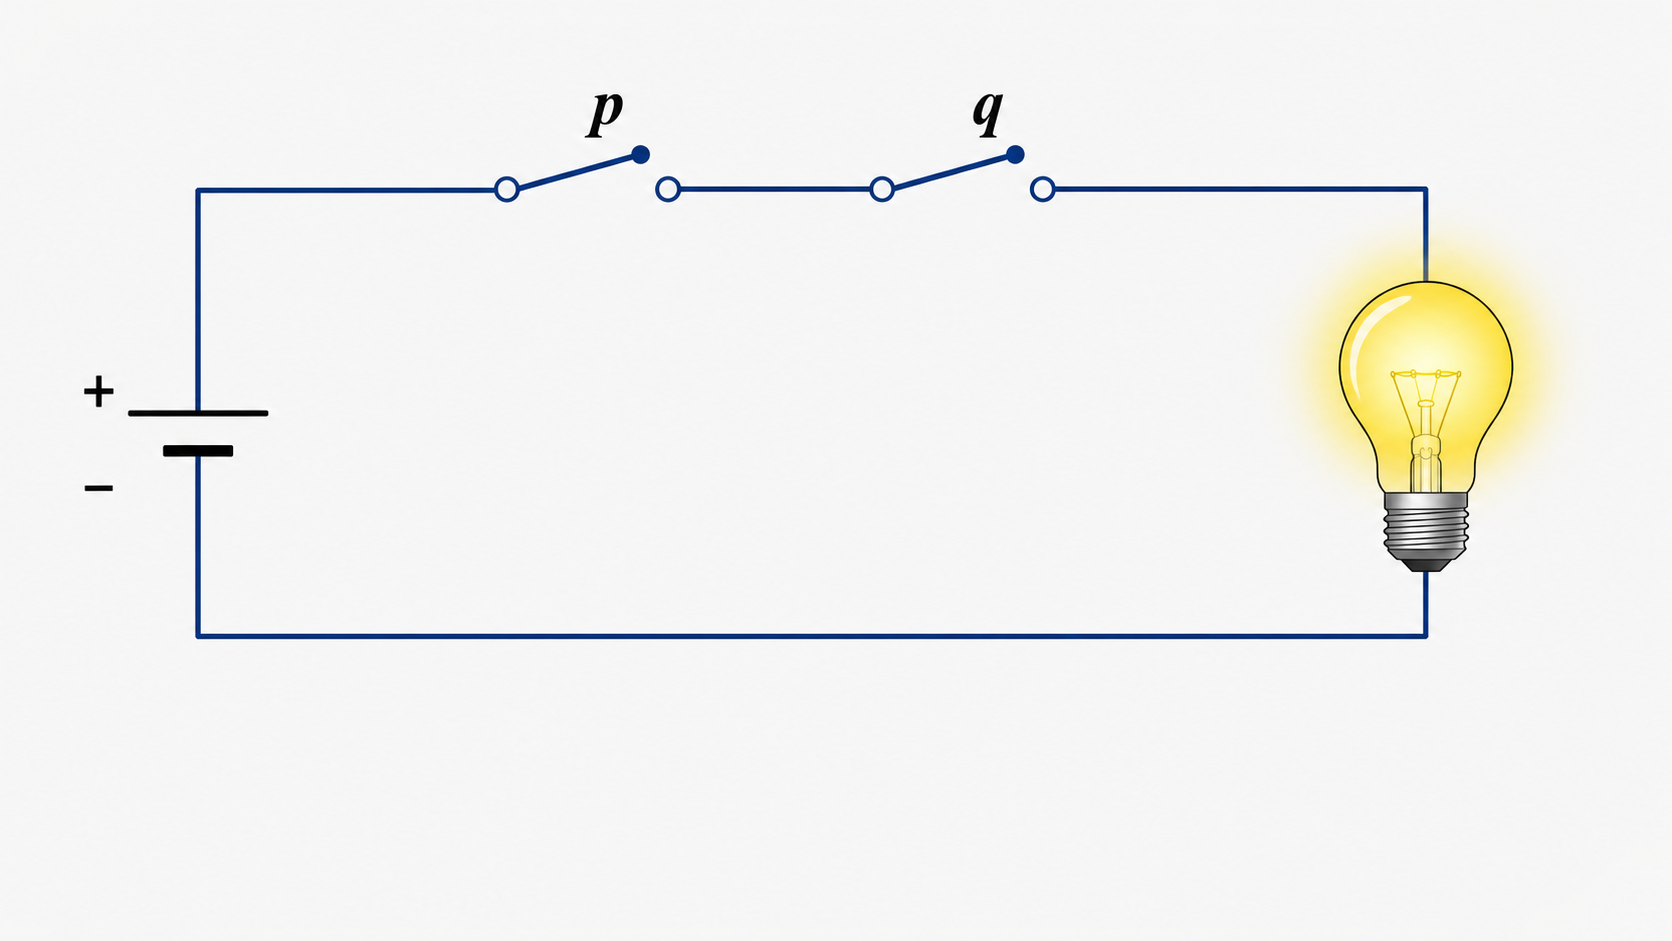
\includegraphics[width=0.8\textwidth]{Figures/02-and-gate-circuit.png}
    \caption{วงจรสวิตช์ไฟฟ้าแบบอนุกรม แสดงการทำงานของ $p \land q$}
    \label{fig:and-gate-circuit}
\end{figure}

\noindent พิจารณาตัวอย่างค่าความจริงของการเชื่อมด้วยคำว่า ``และ'':
\begin{align*}
(2>1) \land (4<5) &\equiv \text{T} \land \text{T} \equiv \text{T}\\
(2+2=5) \land (\text{คนปกติมี 6 ขา}) &\equiv \text{F} \land \text{F} \equiv \text{F}
\end{align*}

\subsection{ประพจน์เลือก (Disjunction / OR, $\lor$)}

ประพจน์เลือก (disjunction, OR) ใช้สัญลักษณ์ $\lor$ ในทางตรรกศาสตร์ และใช้ในวงจรดิจิทัลว่า OR Gate ประพจน์ $p \lor q$ อ่านว่า $p$ หรือ $q$ จะเป็นจริงเมื่อมีอย่างน้อยหนึ่งใน $p$ หรือ $q$ เป็นจริง จะเป็นเท็จก็ต่อเมื่อทั้ง $p$ และ $q$ เป็นเท็จทั้งคู่ ต้องระวังว่า OR ในทางตรรกศาสตร์เป็น OR แบบรวม (Inclusive OR) ซึ่งรวมกรณีที่ทั้งคู่จริงด้วย

\begin{table}[H]
    \centering
    \caption{ประพจน์เลือก ($p \lor q$)}
    \label{tab:or-truth}
    \begin{tabular}{|c|c|c|}
        \hline
        \textbf{$p$} & \textbf{$q$} & \textbf{$p \lor q$} \\ \hline
        T & T & T \\ \hline
        T & F & T \\ \hline
        F & T & T \\ \hline
        F & F & F \\ \hline
    \end{tabular}
\end{table}

\bigskip

\begin{figure}[H]
    \centering
    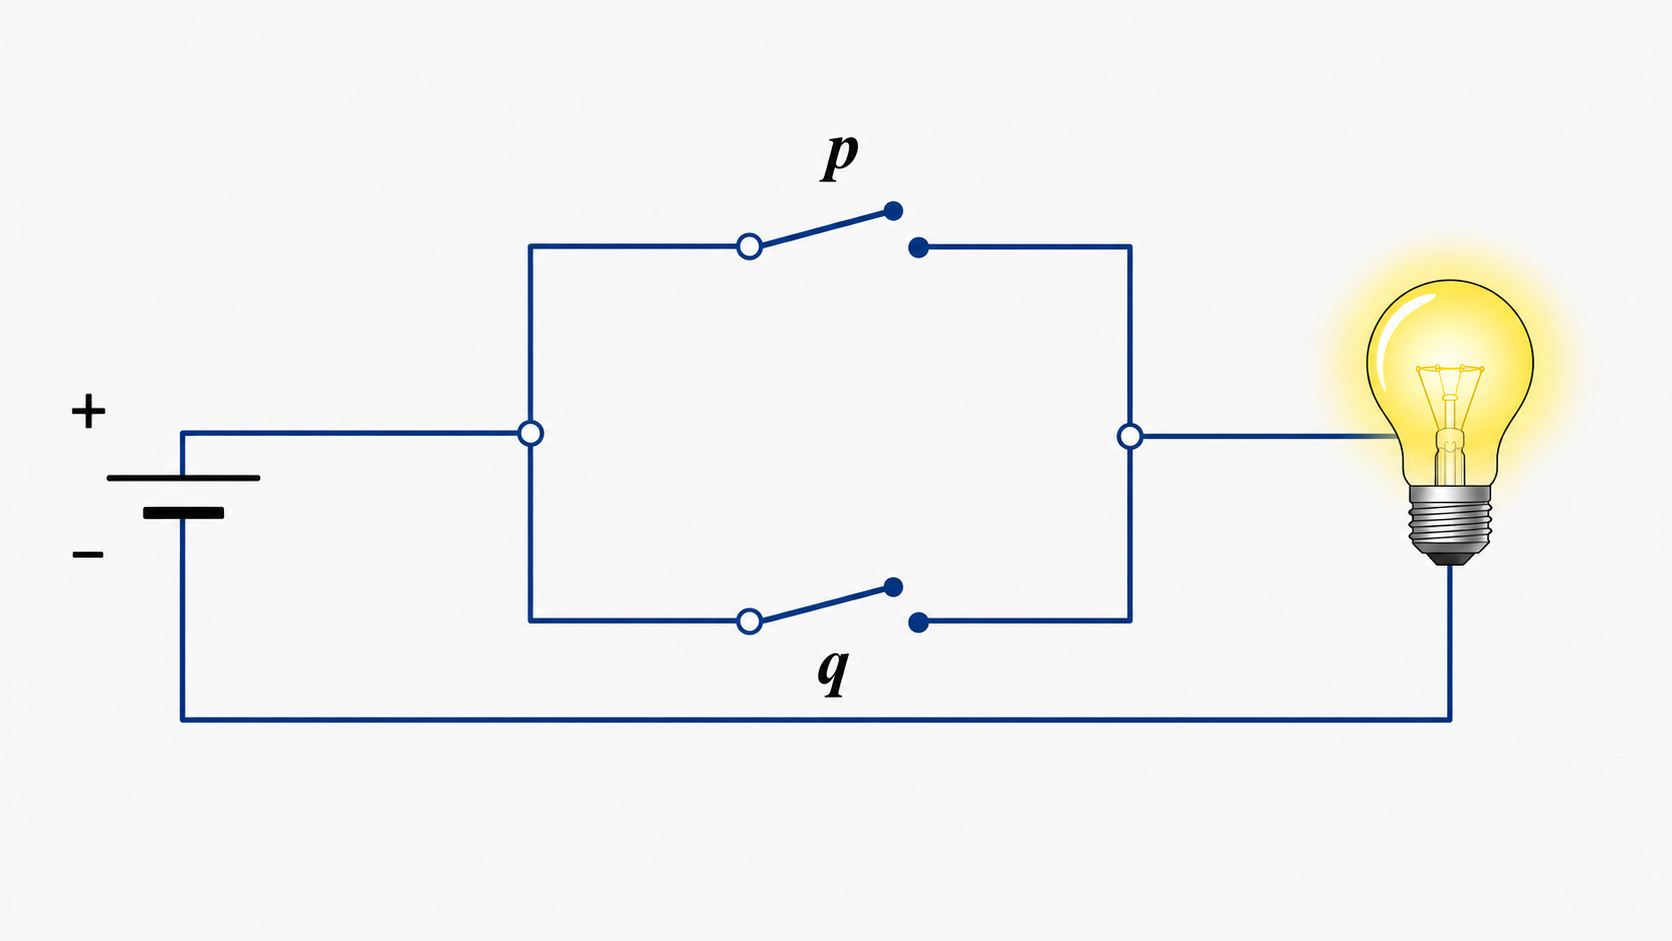
\includegraphics[width=0.8\textwidth]{Figures/03-or-gate-circuit.png}
    \caption{วงจรสวิตช์ไฟฟ้าแบบขนาน แสดงการทำงานของ $p \lor q$}
    \label{fig:or-gate-circuit}
\end{figure}

\noindent พิจารณาตัวอย่างค่าความจริงของการเชื่อมด้วยคำว่า ``หรือ'':
\begin{align*}
(\text{ประเทศไทยอยู่ในทวีปยุโรป}) \lor (2+5>4) &\equiv \text{F} \lor \text{T} \equiv \text{T}\\
(2+2=5) \lor (\text{คนปกติมี 6 ขา}) &\equiv \text{F} \lor \text{F} \equiv \text{F}
\end{align*}

\subsection{นิเสธ (Negation / NOT, $\neg$)}

นิเสธ (Negation) ใช้สัญลักษณ์ $\neg$ เป็นตัวเชื่อมเอกภาพ (Unary Connective) ที่กระทำกับประพจน์เพียงประพจน์เดียว $\neg p$ อ่านว่า ไม่ $p$ หรือ นิเสธของ $p$ การหานิเสธจะกลับค่าความจริงของประพจน์อย่างสมบูรณ์ ถ้า $p$ เป็นจริง $\neg p$ จะเป็นเท็จ และถ้า $p$ เป็นเท็จ $\neg p$ จะเป็นจริง

\begin{table}[H]
    \centering
    \caption{นิเสธ ($\neg p$)}
    \label{tab:not-truth}
    \begin{tabular}{|c|c|}
        \hline
        \textbf{$p$} & \textbf{$\neg p$} \\ \hline
        T & F \\ \hline
        F & T \\ \hline
    \end{tabular}
\end{table}

\subsection{ประพจน์มีเงื่อนไข (Conditional / IMPLIES, $\rightarrow$)}

ประพจน์มีเงื่อนไข (conditional, IMPLIES) ใช้สัญลักษณ์ $\rightarrow$ ประพจน์ $p \rightarrow q$ อ่านว่า ถ้า $p$ แล้ว $q$ โดย $p$ เรียกว่า เงื่อนไขนำ (Antecedent) และ $q$ เรียกว่า เงื่อนไขตาม (Consequent) ค่าความจริงของ $p \rightarrow q$ จะเป็นเท็จเพียงกรณีเดียวคือ เมื่อเงื่อนไขนำ $p$ เป็นจริงแต่เงื่อนไขตาม $q$ เป็นเท็จ

\begin{table}[H]
    \centering
    \caption{ประพจน์มีเงื่อนไข ($p \rightarrow q$)}
    \label{tab:implies-truth}
    \begin{tabular}{|c|c|c|}
        \hline
        \textbf{$p$} & \textbf{$q$} & \textbf{$p \rightarrow q$} \\ \hline
        T & T & T \\ \hline
        T & F & F \\ \hline
        F & T & T \\ \hline
        F & F & T \\ \hline
    \end{tabular}
\end{table}

\bigskip

\begin{figure}[H]
    \centering
    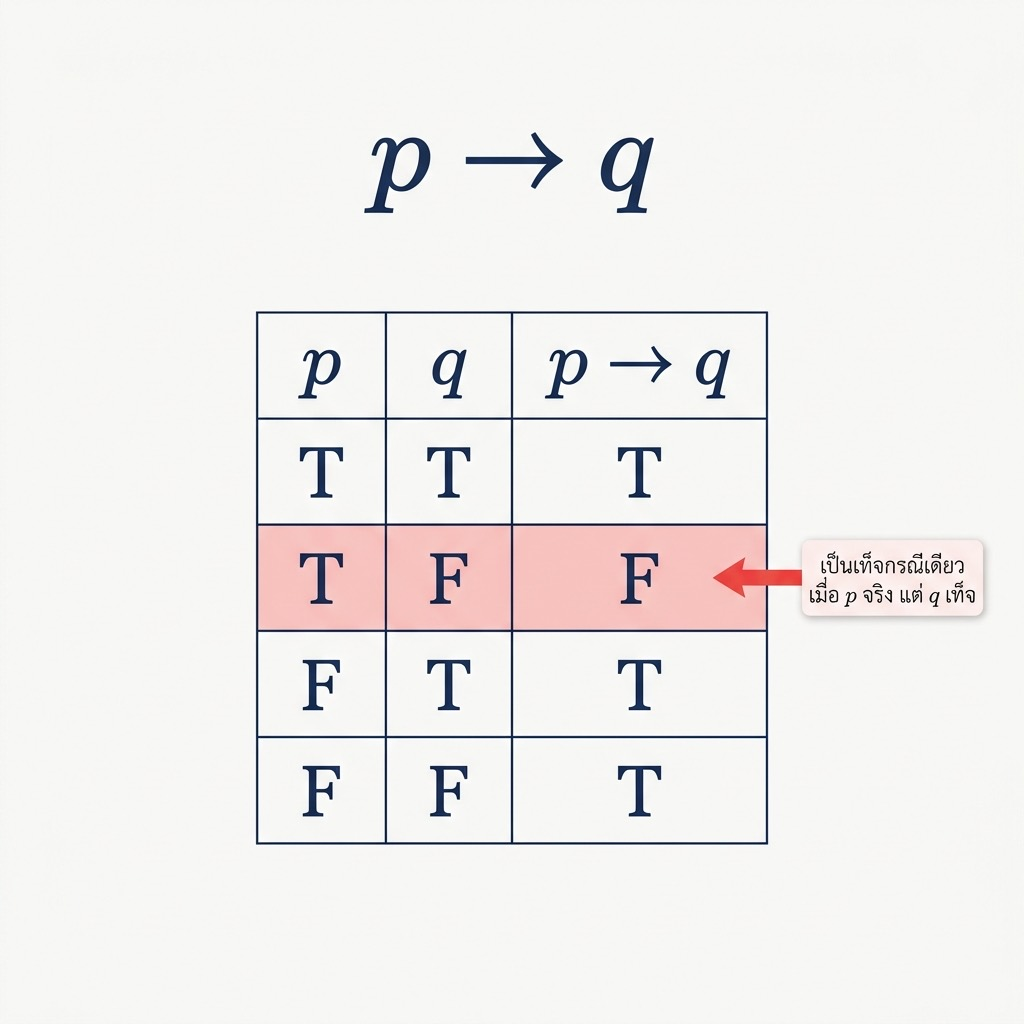
\includegraphics[width=0.8\textwidth]{Figures/04-implication-truth.png}
    \caption{ตารางค่าความจริงของ Implication $p \rightarrow q$ แสดงกรณีที่เป็นเท็จเพียงเมื่อ $p=\text{T}$ แต่ $q=\text{F}$}
    \label{fig:implication-truth}
\end{figure}

\noindent พิจารณาตัวอย่างค่าความจริงของประพจน์มีเงื่อนไข:
\begin{align*}
(\text{เป็นคนปกติ}) \rightarrow (\text{มี 2 ตา}) &\equiv \text{T} \rightarrow \text{T} \equiv \text{T}\\
(\text{เป็นคนปกติ}) \rightarrow (\text{มี 6 ขา}) &\equiv \text{T} \rightarrow \text{F} \equiv \text{F}\\
(\text{หมูบินได้}) \rightarrow (\text{สอบได้ที่หนึ่ง}) &\equiv \text{T} \quad (\text{เงื่อนไขนำเป็นเท็จ})
\end{align*}

\subsection{ประพจน์เงื่อนไขสองทาง (Biconditional / IFF, $\leftrightarrow$)}

ประพจน์เงื่อนไขสองทาง (biconditional, IFF) ใช้สัญลักษณ์ $\leftrightarrow$ ประพจน์ $p \leftrightarrow q$ อ่านว่า ``$p$ ก็ต่อเมื่อ $q$'' หมายความว่า $p$ และ $q$ มีค่าความจริงเหมือนกัน (จริงทั้งคู่หรือเท็จทั้งคู่) IFF เป็นการรวมกันของ $p \rightarrow q$ และ $q \rightarrow p$ ซึ่งสมมูลกับ $(p \rightarrow q) \land (q \rightarrow p)$

\begin{table}[H]
    \centering
    \caption{เงื่อนไขสองทาง ($p \leftrightarrow q$)}
    \label{tab:iff-truth}
    \begin{tabular}{|c|c|c|}
        \hline
        \textbf{$p$} & \textbf{$q$} & \textbf{$p \leftrightarrow q$} \\ \hline
        T & T & T \\ \hline
        T & F & F \\ \hline
        F & T & F \\ \hline
        F & F & T \\ \hline
    \end{tabular}
\end{table}

\bigskip

\noindent พิจารณาตัวอย่างค่าความจริงของการเชื่อมด้วยคำว่า ``ก็ต่อเมื่อ'':
\begin{align*}
(2+2=4) \leftrightarrow (3<5) &\equiv \text{T} \leftrightarrow \text{T} \equiv \text{T}\\
(2+2=5) \leftrightarrow (\text{คนปกติมี 6 ขา}) &\equiv \text{F} \leftrightarrow \text{F} \equiv \text{T}\\
(2+2=4) \leftrightarrow (\text{คนปกติมี 6 ขา}) &\equiv \text{T} \leftrightarrow \text{F} \equiv \text{F}
\end{align*}

\noindent ในทางตรรกศาสตร์ การเชื่อมแบบก็ต่อเมื่อมีความสัมพันธ์อย่างใกล้ชิดกับการเชื่อมแบบถ้า...แล้วสองทิศทาง กล่าวคือ $p \leftrightarrow q$ สมมูลกับ $(p \rightarrow q) \land (q \rightarrow p)$ ความสมมูลนี้มีความสำคัญในการพิสูจน์ทางคณิตศาสตร์และการแปลงประพจน์เชิงตรรกศาสตร์

\begin{prop}
\index{สมมูล!biconditional}
สำหรับทุกประพจน์ $p$ และ $q$ จะได้ว่า
\begin{equation}
p \leftrightarrow q \equiv (p \rightarrow q) \land (q \rightarrow p)
\end{equation}
โดยที่ $p$ และ $q$ เป็นประพจน์ใดๆ, $\rightarrow$ คือตัวเชื่อมแบบถ้า...แล้วที่จะเท็จเพียงกรณีเดียวคือเมื่อเงื่อนไขนำเป็นจริงแต่เงื่อนไขตามเป็นเท็จ และ $\land$ คือตัวเชื่อมแบบและที่จะจริงเมื่อทั้งสองประพจน์เป็นจริง
\end{prop}

\begin{table}[h]
    \centering
    \caption{ตารางพิสูจน์ความสมมูลของ Biconditional}
    \label{tab:biconditional-equiv}
    \begin{tabular}{|c|c|c|c|c|c|}
        \hline
        \textbf{$p$} & \textbf{$q$} & \textbf{$p \rightarrow q$} & \textbf{$q \rightarrow p$} & \textbf{$(p \rightarrow q) \land (q \rightarrow p)$} & \textbf{$p \leftrightarrow q$} \\ \hline
        T & T & T & T & T & T \\ \hline
        T & F & F & T & F & F \\ \hline
        F & T & T & F & F & F \\ \hline
        F & F & T & T & T & T \\ \hline
    \end{tabular}
\end{table}

ตารางที่ \ref{tab:biconditional-equiv} แสดงให้เห็นว่าคอลัมน์ $(p \rightarrow q) \land (q \rightarrow p)$ และ $p \leftrightarrow q$ มีค่าเหมือนกันทุกแถว จึงสรุปได้ว่า $p \leftrightarrow q \equiv (p \rightarrow q) \land (q \rightarrow p)$ ตามที่ต้องการพิสูจน์

\bigskip

\begin{ex}[การหาค่าความจริงของประพจน์]
พิจารณาประพจน์ $(\neg p \land q) \rightarrow r$ จงหาค่าความจริงเมื่อ $p = \text{F}$, $q = \text{T}$, และ $r = \text{F}$
\end{ex}

\begin{solution}
แทนค่า $p = \text{F}$, $q = \text{T}$, และ $r = \text{F}$ ลงในประพจน์เพื่อหาค่าความจริงได้ผลลัพธ์ดังนี้
\begin{align*}
    (\neg p \land q) \rightarrow r &\equiv (\neg \text{F} \land \text{T}) \rightarrow \text{F} \\
    &\equiv (\text{T} \land \text{T}) \rightarrow \text{F} \\
    &\equiv \text{T} \rightarrow \text{F} \\
    &\equiv \text{F}
\end{align*}
ดังนั้น ประพจน์มีค่าความจริงเป็น เท็จ (F)
\end{solution}

\section{สัจนิรันดร์และข้อขัดแย้ง}
\index{สัจนิรันดร์}
\index{Contradiction}
\index{Contingency}
\zlabel{sec:tautology}

เมื่อศึกษาประพจน์เชิงประกอบแล้ว คำถามสำคัญคือ ประพจน์เชิงประกอบนั้นมีค่าความจริงเป็นอย่างไรโดยรวม กล่าวคือ ในทุกกรณีของค่าความจริงของตัวแปรย่อย ประพจน์เชิงประกอบจะมีค่าความจริงเป็นจริงเสมอ หรือเป็นเท็จเสมอ หรือขึ้นกับกรณี การจำแนกประพจน์เชิงประกอบตามลักษณะนี้มีความสำคัญมากในทางคณิตศาสตร์และการพิสูจน์

สัจนิรันดร์ (Tautology) หมายถึง ประพจน์เชิงประกอบที่มีค่าความจริงเป็นจริงในทุกกรณีของการกำหนดค่าความจริงของตัวแปรย่อย ความรู้เรื่องสัจนิรันดร์มีความสำคัญอย่างยิ่งในการพิสูจน์ทางคณิตศาสตร์ เนื่องจากประพจน์ที่เป็นสัจนิรันดร์ถือว่าเป็นความจริงที่จำเป็น (Necessary Truth) ไม่ว่าสถานการณ์จริงเป็นอย่างไรก็ตาม

ในทางตรงกันข้าม ข้อขัดแย้ง (Contradiction) หมายถึง ประพจน์เชิงประกอบที่ไม่มีทางเป็นจริงได้เลย ไม่ว่าค่าความจริงของตัวแปรย่อยจะถูกกำหนดให้เป็นอะไรก็ตาม กล่าวคือ ประพจน์ข้อขัดแย้งจะมีค่าความจริงเป็นเท็จในทุกกรณี ตัวอย่างที่เห็นได้ชัดคือ $p \land \neg p$ ซึ่งสะท้อนหลักการที่ว่า $p$ กับ $\neg p$ ไม่อาจเป็นจริงพร้อมกันได้

สำหรับประพจน์กลาง (Contingency) คือ ประพจน์เชิงประกอบที่มีค่าความจริงเป็นจริงบ้างและเป็นเท็จบ้าง ขึ้นอยู่กับค่าของตัวแปรย่อย ประพจน์ส่วนใหญ่ในชีวิตจริงเป็นประพจน์กลาง

\subsection{สัจนิรันดร์ (Tautology)}
ประพจน์เชิงประกอบบางรูปแบบให้ค่าความจริงเป็นจริงทุกแถวของตารางค่าความจริง ไม่ว่าจะแทนค่าตัวแปรย่อยด้วยจริงหรือเท็จอย่างไร ประพจน์ลักษณะนี้เรียกว่าสัจนิรันดร์

\begin{definition}[สัจนิรันดร์]
\index{สัจนิรันดร์!นิยาม}
สัจนิรันดร์ (Tautology) คือ ประพจน์เชิงประกอบที่มีค่าความจริงเป็นจริงในทุกกรณีของการกำหนดค่าความจริงของตัวแปรย่อย
\end{definition}

ตัวอย่างที่ง่ายที่สุดของสัจนิรันดร์คือ $p \lor \neg p$ ซึ่งอ่านว่า $p$ หรือไม่ $p$ ประพจน์นี้เป็นจริงเสมอ เนื่องจากในทุกสถานการณ์ $p$ จะต้องเป็นจริงหรือเท็จอย่างใดอย่างหนึ่ง จึงทำให้ $p \lor \neg p$ เป็นจริงในทุกกรณี ผลลัพธ์นี้สอดคล้องกับกฎกีดกันกลาง (Law of Excluded Middle) ของอริสโตเติล~\cite{aristotle_organon} ซึ่งระบุว่าสำหรับทุกประพจน์ $p$ แล้ว $p$ หรือ $\neg p$ จะต้องเป็นจริงอย่างน้อยหนึ่งอย่าง

\begin{table}[h]
    \centering
    \caption{ตารางแสดงว่า $p \lor \neg p$ เป็นสัจนิรันดร์}
    \label{tab:tautology-law-excluded}
    \begin{tabular}{|c|c|c|}
        \hline
        \textbf{$p$} & \textbf{$\neg p$} & \textbf{$p \lor \neg p$} \\ \hline
        T & F & T \\ \hline
        F & T & T \\ \hline
    \end{tabular}
\end{table}

ตารางที่ \ref{tab:tautology-law-excluded} แสดงให้เห็นว่าคอลัมน์สุดท้ายมีค่า T ทุกแถว จึงเป็นสัจนิรันดร์

ตัวอย่างสัจนิรันดร์อื่นๆ ได้แก่ $p \rightarrow p$ ซึ่งหมายความว่าถ้า $p$ แล้ว $p$ ย่อมจริงเสมอ $p \leftrightarrow p$ ซึ่งหมายความว่า $p$ ก็ต่อเมื่อ $p$ และ $(p \land q) \rightarrow p$ ซึ่งหมายความว่าถ้า $p$ และ $q$ เป็นจริง แล้ว $p$ ย่อมจริง

\begin{table}[h]
    \centering
    \caption{ตารางแสดงว่า $(p \land q) \rightarrow p$ เป็นสัจนิรันดร์}
    \label{tab:tautology-absorption}
    \begin{tabular}{|c|c|c|c|c|}
        \hline
        \textbf{$p$} & \textbf{$q$} & \textbf{$p \land q$} & \textbf{$(p \land q) \rightarrow p$} & \textbf{ผลลัพธ์} \\ \hline
        T & T & T & T & T \\ \hline
        T & F & F & T & T \\ \hline
        F & T & F & T & T \\ \hline
        F & F & F & T & T \\ \hline
    \end{tabular}
\end{table}

ตารางที่ \ref{tab:tautology-absorption} แสดงให้เห็นว่า $(p \land q) \rightarrow p$ เป็นจริงทุกกรณี

การพิสูจน์โดยการใช้สัจนิรันดร์ ในการพิสูจน์ทางคณิตศาสตร์ หากต้องการแสดงว่าข้อความ $P$ เป็นจริง อาจพิสูจน์ว่า $\neg P$ นำไปสู่ข้อขัดแย้ง (Contradiction) เมื่อ $\neg P$ นำไปสู่ข้อขัดแย้ง แสดงว่า $\neg P$ เป็นเท็จ จึงสรุปได้ว่า $P$ เป็นจริง วิธีนี้เรียกว่า การพิสูจน์โดยข้อขัดแย้ง (Proof by Contradiction) ตัวอย่างต่อไปนี้เป็นตัวอย่างคลาสสิกที่ใช้เทคนิคดังกล่าว จึงควรอ่านในฐานะสะพานเชื่อมระหว่างตรรกศาสตร์กับวิธีพิสูจน์ทางคณิตศาสตร์

\begin{ex}[การพิสูจน์โดยข้อขัดแย้ง]
จงพิสูจน์ว่า $\sqrt{2}$ เป็นจำนวนอตรรกยะ
\end{ex}

\begin{solution}
สมมติในทางตรงข้ามว่า $\sqrt{2}$ เป็นจำนวนตรรกยะ จะเขียนได้เป็น $\sqrt{2} = \dfrac{a}{b}$ โดย $a,b \in \mathbb{Z}$, $b \neq 0$ และ $\gcd(a,b)=1$
\begin{align*}
\sqrt{2} = \frac{a}{b} \ &\Rightarrow\ 2 = \frac{a^2}{b^2} \ \Rightarrow\ a^2 = 2b^2 \quad (a^2 \text{ คู่} \Rightarrow a \text{ คู่})\\
a = 2c \ &\Rightarrow\ (2c)^2 = 2b^2 \ \Rightarrow\ b^2 = 2c^2 \quad (b^2 \text{ คู่} \Rightarrow b \text{ คู่})
\end{align*}
แต่ $a$ และ $b$ เป็นจำนวนคู่ทั้งคู่ ขัดแย้งกับ $\gcd(a,b)=1$ ดังนั้นข้อสมมติเป็นเท็จ จึงสรุปว่า $\sqrt{2}$ เป็นจำนวนอตรรกยะ \solhere
\end{solution}

การพิสูจน์นี้ใช้หลักการว่า ถ้า $\neg P$ นำไปสู่ข้อขัดแย้ง แสดงว่า $P$ เป็นจริง

\subsection{ข้อขัดแย้ง (Contradiction)}
ในทางกลับกัน ประพจน์เชิงประกอบบางรูปแบบให้ค่าความจริงเป็นเท็จทุกแถวของตารางค่าความจริง ไม่ว่าจะแทนค่าตัวแปรย่อยอย่างไร ประพจน์ลักษณะนี้เรียกว่าข้อขัดแย้ง

\begin{definition}[ข้อขัดแย้ง]
\index{ข้อขัดแย้ง!นิยาม}
ข้อขัดแย้ง (Contradiction) คือ ประพจน์เชิงประกอบที่ไม่มีทางเป็นจริงได้ ไม่ว่าค่าความจริงของตัวแปรย่อยจะถูกกำหนดให้เป็นอะไรก็ตาม ประพจน์ที่เป็นข้อขัดแย้งจะมีค่าความจริงเป็นเท็จเสมอ
\end{definition}

ตัวอย่างที่ง่ายที่สุดของข้อขัดแย้งคือ $p \land \neg p$ ซึ่งอ่านว่า $p$ และไม่ $p$ ประพจน์นี้เป็นเท็จเสมอ เนื่องจากประพจน์เดียวกันไม่อาจมีค่าความจริงเป็นทั้งจริงและเท็จในเวลาเดียวกันได้

หลักการนี้สอดคล้องกับกฎแห่งการไม่ขัดแย้ง (Law of Non-Contradiction) ซึ่งระบุว่า $p$ กับ $\neg p$ ไม่อาจเป็นจริงพร้อมกันได้ การเข้าใจข้อขัดแย้งมีความสำคัญในการพิสูจน์ทางคณิตศาสตร์ เนื่องจากเมื่อแสดงว่าข้อสันนิษฐานหนึ่งนำไปสู่ข้อขัดแย้ง ย่อมสรุปได้ว่าข้อสันนิษฐานนั้นต้องเป็นเท็จ

\begin{table}[h]
    \centering
    \caption{ตารางแสดงว่า $p \land \neg p$ เป็นข้อขัดแย้ง}
    \label{tab:contradiction}
    \begin{tabular}{|c|c|c|c|}
        \hline
        \textbf{$p$} & \textbf{$\neg p$} & \textbf{$p \land \neg p$} & \textbf{ผลลัพธ์} \\ \hline
        T & F & F & F \\ \hline
        F & T & F & F \\ \hline
    \end{tabular}
\end{table}

ตารางที่ \ref{tab:contradiction} แสดงให้เห็นว่าคอลัมน์สุดท้ายมีค่า F ทุกแถว จึงเป็นข้อขัดแย้ง

ตัวอย่างข้อขัดแย้งอื่นๆ ได้แก่ $\neg(p \lor \neg p)$ ซึ่งเป็นนิเสธของกฎกีดกันกลาง และ $(p \rightarrow q) \land (p \land \neg q)$ ซึ่งหมายความว่า $q$ ต้องเป็นจริงและเท็จพร้อมกันภายใต้เงื่อนไขเดียวกัน

หากพบว่าการสันนิษฐานนำไปสู่ข้อขัดแย้ง แสดงว่าการสันนิษฐานนั้นเป็นเท็จ นี่คือหลักการพื้นฐานของการพิสูจน์โดยข้อขัดแย้ง (Proof by Contradiction) ซึ่งเป็นเทคนิคพื้นฐานในทางคณิตศาสตร์

ความสัมพันธ์ระหว่างสัจนิรันดร์และข้อขัดแย้งมีความสำคัญ โดยนิเสธของสัจนิรันดร์คือข้อขัดแย้ง และนิเสธของข้อขัดแย้งคือสัจนิรันดร์ กล่าวคือ ถ้า $P$ เป็นสัจนิรันดร์ แล้ว $\neg P$ จะเป็นข้อขัดแย้ง และถ้า $P$ เป็นข้อขัดแย้ง แล้ว $\neg P$ จะเป็นสัจนิรันดร์

\subsection{ประพจน์กลาง (Contingency)}

ประพจน์กลาง (Contingency) คือ ประพจน์เชิงประกอบที่มีค่าความจริงเป็นจริงบ้างและเป็นเท็จบ้าง ขึ้นอยู่กับค่าความจริงของตัวแปรย่อย กล่าวคือ ไม่เป็นสัจนิรันดร์ก็ไม่เป็นข้อขัดแย้ง แต่มีค่าความจริงขึ้นกับการกำหนดค่าของตัวแปรย่อย ประพจน์ส่วนใหญ่ในชีวิตประจำวันและในคณิตศาสตร์เป็นประพจน์กลาง

\begin{table}[h]
    \centering
    \caption{ตารางแสดงว่า $p \land q$ เป็นประพจน์กลาง}
    \label{tab:contingency-example}
    \begin{tabular}{|c|c|c|c|}
        \hline
        \textbf{$p$} & \textbf{$q$} & \textbf{$p \land q$} & \textbf{ผลลัพธ์} \\ \hline
        T & T & T & T \\ \hline
        T & F & F & F \\ \hline
        F & T & F & F \\ \hline
        F & F & F & F \\ \hline
    \end{tabular}
\end{table}

ตารางที่ \ref{tab:contingency-example} แสดงให้เห็นว่า $p \land q$ ไม่เป็นสัจนิรันดร์ (เพราะมี F) และไม่เป็นข้อขัดแย้ง (เพราะมี T) จึงเป็นประพจน์กลาง

ประพจน์กลางเป็นประพจน์ที่มีความหมายจริงในการใช้งาน เนื่องจากค่าความจริงของประพจน์กลางขึ้นกับข้อเท็จจริงในโลกจริง ตัวอย่างเช่น ประพจน์ วันนี้ฝนตก จะเป็นจริงหรือเท็จขึ้นกับสถานการณ์จริงในวันนั้น

\section{ความสมมูลเชิงตรรกะและกฎพีชคณิตของประพจน์}
\index{ความสมมูลเชิงตรรกะ}
\index{Logical Equivalence}
\label{sec:logical-equivalence}

ในการวิเคราะห์และจัดรูปประพจน์เชิงประกอบ มักพบว่าประพจน์ที่มีรูปแบบสัญลักษณ์แตกต่างกันอาจให้ค่าความจริงเหมือนกันในทุกกรณี ความสัมพันธ์นี้เรียกว่า ความสมมูลเชิงตรรกะ (Logical Equivalence) ซึ่งเป็นแนวคิดที่สำคัญทั้งในการพิสูจน์ทางคณิตศาสตร์ การลดรูปนิพจน์บูลีน และการออกแบบวงจรดิจิทัล

\begin{definition}[ความสมมูลเชิงตรรกะ]
\index{ความสมมูลเชิงตรรกะ!นิยาม}
ประพจน์ $P$ และ $Q$ เรียกว่า สมมูลเชิงตรรกะ (Logically Equivalent) เขียนแทนด้วย $P \equiv Q$ ก็ต่อเมื่อ $P$ และ $Q$ มีค่าความจริงเหมือนกันในทุกกรณีของการกำหนดค่าความจริงของตัวแปรย่อย หรือกล่าวอย่างเทียบเท่าว่า ประพจน์ $P \leftrightarrow Q$ เป็นสัจนิรันดร์
\end{definition}

จากนิยามจะเห็นได้ว่า การตรวจสอบความสมมูลทำได้สองวิธีหลัก คือ สร้างตารางค่าความจริงเปรียบเทียบทีละแถว หรือใช้กฎพีชคณิตของประพจน์ในการแปลงรูปจากด้านหนึ่งให้กลายเป็นอีกด้านหนึ่ง

\subsection{กฎพีชคณิตของประพจน์ (Laws of Propositional Algebra)}
\index{พีชคณิตของประพจน์}

กฎพีชคณิตของประพจน์เป็นชุดของความสมมูลพื้นฐานที่ใช้บ่อยในการลดรูปและพิสูจน์ทฤษฎีบทเชิงตรรกะ อันที่จริงกฎเหล่านี้เป็น \emph{กรณีรูปธรรม} ของกฎในพีชคณิตบูลีน (Boolean Algebra) ซึ่งเป็นโครงสร้างนามธรรมที่จะได้ศึกษาอย่างละเอียดใน\autoref{ch:boolean} (กฎชุดเดียวกันนี้ยังปรากฏในทฤษฎีเซตอีกด้วย ดังจะเห็นใน\autoref{ch:set}) ตารางที่ \ref{tab:propositional-laws} สรุปกฎที่สำคัญทั้งหมด

\begin{table}[h]
    \centering
    \caption{กฎพีชคณิตของประพจน์ (โดยที่ $T$ แทนสัจนิรันดร์ และ $F$ แทนข้อขัดแย้ง)}
    \label{tab:propositional-laws}
    \begin{tabular}{|l|l|}
        \hline
        \textbf{ชื่อกฎ} & \textbf{รูปสมมูล} \\ \hline
        กฎเอกลักษณ์ (Identity) & $p \land T \equiv p$, \quad $p \lor F \equiv p$ \\ \hline
        กฎครอบงำ (Domination) & $p \lor T \equiv T$, \quad $p \land F \equiv F$ \\ \hline
        กฎนิจพล (Idempotent) & $p \lor p \equiv p$, \quad $p \land p \equiv p$ \\ \hline
        กฎนิเสธซ้อน (Double Negation) & $\neg(\neg p) \equiv p$ \\ \hline
        กฎสลับที่ (Commutative) & $p \lor q \equiv q \lor p$, \quad $p \land q \equiv q \land p$ \\ \hline
        กฎเปลี่ยนกลุ่ม (Associative) & $(p \lor q) \lor r \equiv p \lor (q \lor r)$ \\ \hline
                                     & $(p \land q) \land r \equiv p \land (q \land r)$ \\ \hline
        กฎแจกแจง (Distributive) & $p \lor (q \land r) \equiv (p \lor q) \land (p \lor r)$ \\ \hline
                                & $p \land (q \lor r) \equiv (p \land q) \lor (p \land r)$ \\ \hline
        กฎเดอมอร์แกน (De Morgan) & $\neg(p \land q) \equiv \neg p \lor \neg q$ \\ \hline
                                 & $\neg(p \lor q) \equiv \neg p \land \neg q$ \\ \hline
        กฎดูดกลืน (Absorption) & $p \lor (p \land q) \equiv p$, \quad $p \land (p \lor q) \equiv p$ \\ \hline
        กฎนิเสธ (Negation) & $p \lor \neg p \equiv T$, \quad $p \land \neg p \equiv F$ \\ \hline
        กฎเงื่อนไข (Implication) & $p \rightarrow q \equiv \neg p \lor q$ \\ \hline
        กฎกระจายเงื่อนไข (Exportation) & $(p \land q) \rightarrow r \equiv p \rightarrow (q \rightarrow r)$ \\ \hline
    \end{tabular}
\end{table}

ตารางที่ \ref{tab:propositional-laws} สรุปกฎพื้นฐานของพีชคณิตของประพจน์ที่ใช้บ่อยที่สุด กฎเหล่านี้สามารถพิสูจน์ได้ทุกข้อด้วยตารางค่าความจริง และจะถูกนำไปใช้ใน\autoref{ch:boolean} (พีชคณิตบูลีน) เพื่อออกแบบและลดรูปวงจรดิจิทัล

\begin{ex}[การใช้กฎพีชคณิตในการลดรูป]
จงพิสูจน์ว่า $\neg(p \lor q) \lor (\neg p \land q) \equiv \neg p$ โดยใช้กฎพีชคณิตของประพจน์
\end{ex}

\begin{solution}
\begin{align*}
\neg(p \lor q) \lor (\neg p \land q) &\equiv (\neg p \land \neg q) \lor (\neg p \land q) \quad \text{(กฎเดอมอร์แกน)} \\
&\equiv \neg p \land (\neg q \lor q) \quad \text{(กฎแจกแจง)} \\
&\equiv \neg p \land T \quad \text{(กฎนิเสธ)} \\
&\equiv \neg p \quad \text{(กฎเอกลักษณ์)}
\end{align*}
ดังนั้น $\neg(p \lor q) \lor (\neg p \land q) \equiv \neg p$
\end{solution}

\subsection{ประพจน์กลับ ประพจน์ผกผัน และประพจน์แย้งสลับที่ (Converse, Inverse, Contrapositive)}
\index{Converse}
\index{Inverse}
\index{Contrapositive}
\index{ผกผัน}
\index{แย้งสลับที่}

ประพจน์เงื่อนไข $p \rightarrow q$ มีประพจน์ที่เกี่ยวข้องกันอย่างใกล้ชิดอีกสามรูปแบบ ซึ่งใช้ในการพิสูจน์ทางคณิตศาสตร์ โดยเฉพาะการพิสูจน์โดยแย้งสลับที่ (Proof by Contrapositive)

\begin{definition}[Converse, Inverse, Contrapositive]
\index{ประพจน์เงื่อนไข!converse}
กำหนดประพจน์เงื่อนไข $p \rightarrow q$
\begin{itemize}
    \item ส่วนกลับ (Converse) คือ $q \rightarrow p$
    \item ผกผัน (Inverse) คือ $\neg p \rightarrow \neg q$
    \item แย้งสลับที่ (Contrapositive) คือ $\neg q \rightarrow \neg p$
\end{itemize}
\end{definition}

ความสัมพันธ์ที่สำคัญที่สุดของประพจน์ทั้งสี่นี้คือ ประพจน์เงื่อนไขกับแย้งสลับที่สมมูลกันเสมอ ในขณะที่ส่วนกลับและผกผันก็สมมูลกันเสมอ แต่ประพจน์เงื่อนไขกับส่วนกลับ \textbf{ไม่สมมูล} กันโดยทั่วไป การสับสนระหว่างประพจน์เงื่อนไขกับส่วนกลับเป็นข้อผิดพลาดเชิงตรรกะที่พบบ่อย (เรียกว่า Affirming the Consequent)

\begin{table}[h]
    \centering
    \caption{ตารางพิสูจน์ความสมมูลของประพจน์เงื่อนไขและแย้งสลับที่}
    \label{tab:contrapositive}
    \begin{tabular}{|c|c|c|c|c|c|}
        \hline
        \textbf{$p$} & \textbf{$q$} & \textbf{$\neg p$} & \textbf{$\neg q$} & \textbf{$p \rightarrow q$} & \textbf{$\neg q \rightarrow \neg p$} \\ \hline
        T & T & F & F & T & T \\ \hline
        T & F & F & T & F & F \\ \hline
        F & T & T & F & T & T \\ \hline
        F & F & T & T & T & T \\ \hline
    \end{tabular}
\end{table}

ตารางที่ \ref{tab:contrapositive} แสดงให้เห็นว่า $p \rightarrow q$ และ $\neg q \rightarrow \neg p$ มีค่าความจริงเหมือนกันทุกแถว จึงสรุปได้ว่า $p \rightarrow q \equiv \neg q \rightarrow \neg p$

\begin{ex}[การเขียน Converse, Inverse, Contrapositive]
กำหนดประพจน์ ``ถ้า $n$ เป็นจำนวนเฉพาะที่มากกว่า 2 แล้ว $n$ เป็นจำนวนคี่'' จงเขียนส่วนกลับ ผกผัน และแย้งสลับที่ของประพจน์นี้
\end{ex}

\begin{solution}
ให้ $p \equiv $ ``$n$ เป็นจำนวนเฉพาะที่มากกว่า 2'' และ $q \equiv$ ``$n$ เป็นจำนวนคี่''
\begin{itemize}
    \item ส่วนกลับ ถ้า $n$ เป็นจำนวนคี่ แล้ว $n$ เป็นจำนวนเฉพาะที่มากกว่า 2 \quad (เป็นเท็จ เช่น $n=9$)
    \item ผกผัน ถ้า $n$ ไม่เป็นจำนวนเฉพาะที่มากกว่า 2 แล้ว $n$ ไม่เป็นจำนวนคี่ \quad (เป็นเท็จ เช่น $n=9$)
    \item แย้งสลับที่ ถ้า $n$ ไม่เป็นจำนวนคี่ แล้ว $n$ ไม่เป็นจำนวนเฉพาะที่มากกว่า 2 \quad (เป็นจริง สมมูลกับประพจน์เดิม)
\end{itemize}
\end{solution}

\section{ตัวเชื่อมเพิ่มเติม: XOR, NAND, NOR}
\index{XOR}
\index{NAND}
\index{NOR}
\zlabel{sec:extended-connectives}

นอกจากตัวเชื่อมพื้นฐาน 5 ตัวที่ได้ศึกษามาแล้ว ยังมีตัวเชื่อมอีกหลายตัวที่นิยมใช้ในวงจรดิจิทัลและวิทยาการคอมพิวเตอร์ ตัวเชื่อมเหล่านี้สามารถนิยามได้จากตัวเชื่อมพื้นฐาน 5 ตัว แต่การมีสัญลักษณ์เฉพาะช่วยให้การเขียนนิพจน์กระชับและเข้าใจง่ายขึ้น

\subsection{ประพจน์เลือกเฉพาะ (Exclusive OR, XOR, $\oplus$)}
\index{XOR!Exclusive OR}

Exclusive OR หรือเรียกย่อว่า XOR ใช้สัญลักษณ์ $\oplus$ เป็นตัวเชื่อมที่ให้ค่าจริงเมื่อประพจน์ทั้งสองมีค่าความจริงต่างกันเท่านั้น แตกต่างจาก OR แบบรวม (Inclusive OR, $\lor$) ที่อนุญาตให้ทั้งคู่เป็นจริงได้ XOR เป็นแบบจำลองเชิงตรรกะของคำว่า ``หรือ'' ในความหมายที่ \textit{เลือกได้อย่างใดอย่างหนึ่งเท่านั้น}

\begin{definition}[Exclusive OR]
\index{XOR!นิยาม}
สำหรับประพจน์ $p$ และ $q$ ใดๆ ประพจน์ $p \oplus q$ มีค่าความจริงเป็นจริงก็ต่อเมื่อ $p$ และ $q$ มีค่าความจริงต่างกัน และเป็นเท็จเมื่อ $p$ กับ $q$ มีค่าความจริงเหมือนกัน หรือเขียนในรูปสมมูลได้ว่า
\begin{equation}
p \oplus q \equiv (p \lor q) \land \neg(p \land q) \equiv (p \land \neg q) \lor (\neg p \land q)
\end{equation}
\end{definition}

\begin{figure}[H]
    \centering
    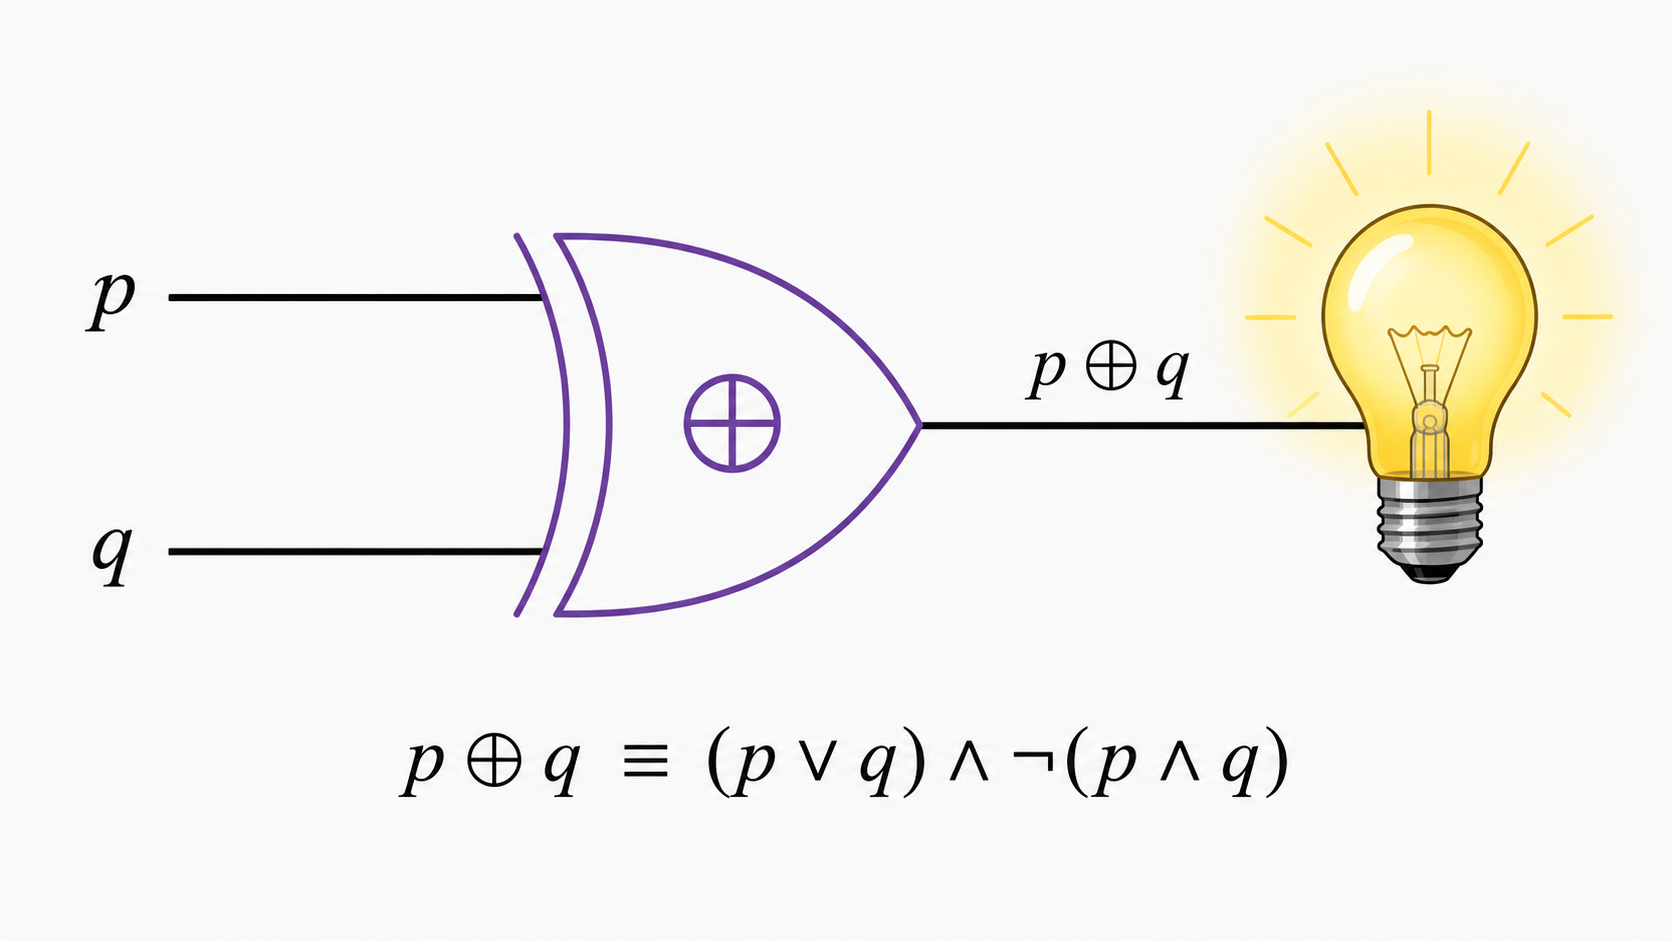
\includegraphics[width=0.85\textwidth]{Figures/09-xor-logic.png}
    \caption{ตารางค่าความจริงและสัญลักษณ์ของลอจิกเกต XOR}
    \label{fig:xor-logic}
\end{figure}

รูปที่ \ref{fig:xor-logic} แสดงตารางค่าความจริงและสัญลักษณ์ของลอจิกเกต XOR ซึ่งให้ผลลัพธ์เป็นจริงเฉพาะเมื่ออินพุตทั้งสองต่างกัน

\begin{table}[h]
    \centering
    \caption{ตารางค่าความจริงของ XOR ($p \oplus q$)}
    \label{tab:xor-truth}
    \begin{tabular}{|c|c|c|}
        \hline
        \textbf{$p$} & \textbf{$q$} & \textbf{$p \oplus q$} \\ \hline
        T & T & F \\ \hline
        T & F & T \\ \hline
        F & T & T \\ \hline
        F & F & F \\ \hline
    \end{tabular}
\end{table}

XOR ใช้ในวิทยาการคอมพิวเตอร์หลายด้าน เช่น
\begin{enumerate}
    \item วงจรบวกเลขฐานสอง (Binary Adder) วงจร Half-Adder ใช้ XOR ในการคำนวณบิตผลรวม (sum bit) ส่วนค่าทด (carry) คำนวณจาก AND
    \item การเข้ารหัสลับ (Cryptography) XOR ถูกนำมาใช้ใน Stream Cipher และ One-Time Pad เพราะมีคุณสมบัติย้อนกลับได้ในตัวเอง กล่าวคือ ถ้า $C = M \oplus K$ แล้ว $M = C \oplus K$ เมื่อ $M$ คือข้อความ $K$ คือกุญแจ และ $C$ คือข้อความที่เข้ารหัสแล้ว
    \item การตรวจสอบความถูกต้องของข้อมูล (Parity Check) ใช้ XOR ของบิตทั้งหมดเพื่อสร้างบิตตรวจสอบ (parity bit) สำหรับตรวจจับความผิดพลาดในการส่งข้อมูล
    \item การสลับค่าตัวแปร (Swap without Temporary Variable) เทคนิคในการเขียนโปรแกรมที่สลับค่าระหว่างตัวแปรสองตัวโดยไม่ใช้ตัวแปรชั่วคราว ผ่านการประยุกต์ XOR สามครั้ง
\end{enumerate}

\subsection{แนนด์และนอร์ (NAND $\uparrow$, NOR $\downarrow$)}
\index{NAND}
\index{NOR}
\index{Universal Gate}

NAND และ NOR เป็นนิเสธของ AND และ OR ตามลำดับ จุดเด่นของตัวเชื่อมทั้งสองคือ คุณสมบัติเป็น \textbf{ตัวเชื่อมสากล (Universal Connective)} หรือในวงจรดิจิทัลเรียกว่า \textbf{Universal Gate} กล่าวคือ สามารถใช้ NAND เพียงอย่างเดียว หรือ NOR เพียงอย่างเดียว ในการสร้างตัวเชื่อมพื้นฐานทั้งหมด (NOT, AND, OR) และจึงสร้างวงจรดิจิทัลใดๆ ก็ได้ คุณสมบัตินี้เป็นเหตุผลสำคัญที่ทำให้การผลิตชิปนิยมใช้ NAND gate เป็นหลัก เพราะลดความซับซ้อนของกระบวนการผลิต

\begin{definition}[NAND และ NOR]
\index{NAND!นิยาม}
\index{NOR!นิยาม}
สำหรับประพจน์ $p$ และ $q$ ใดๆ
\begin{align*}
p \uparrow q &\equiv \neg(p \land q) \quad \text{(NAND, Sheffer stroke)} \\
p \downarrow q &\equiv \neg(p \lor q) \quad \text{(NOR, Peirce arrow)}
\end{align*}
\end{definition}

\begin{table}[h]
    \centering
    \caption{ตารางค่าความจริงของ NAND และ NOR}
    \label{tab:nand-nor-truth}
    \begin{tabular}{|c|c|c|c|}
        \hline
        \textbf{$p$} & \textbf{$q$} & \textbf{$p \uparrow q$ (NAND)} & \textbf{$p \downarrow q$ (NOR)} \\ \hline
        T & T & F & F \\ \hline
        T & F & T & F \\ \hline
        F & T & T & F \\ \hline
        F & F & T & T \\ \hline
    \end{tabular}
\end{table}

ตารางที่ \ref{tab:nand-nor-truth} แสดงค่าความจริงของ NAND และ NOR สังเกตว่า NAND เป็นเท็จเพียงกรณีเดียวคือเมื่อ $p$ และ $q$ จริงทั้งคู่ ส่วน NOR เป็นจริงเพียงกรณีเดียวคือเมื่อ $p$ และ $q$ เท็จทั้งคู่

ตัวอย่างการสร้าง NOT จาก NAND เพียงอย่างเดียว: $\neg p \equiv p \uparrow p$ เพราะ $p \uparrow p \equiv \neg(p \land p) \equiv \neg p$ และการสร้าง AND จาก NAND ทำได้โดย $p \land q \equiv (p \uparrow q) \uparrow (p \uparrow q)$ รายละเอียดของการประยุกต์เพิ่มเติมและการออกแบบวงจรลอจิกจะกล่าวถึงใน\autoref{ch:boolean} ว่าด้วยพีชคณิตบูลีน

\section{ประพจน์เปิดและตัวบ่งปริมาณ (Predicates and Quantifiers)}
\index{ตัวบ่งปริมาณ}
\index{Quantifiers}
\index{ประพจน์เปิด}

ประพจน์ที่ศึกษามาทั้งหมดเป็นประโยคที่ระบุค่าความจริงได้แน่นอน แต่ในทางคณิตศาสตร์เรามักพบประโยคที่มีตัวแปร เช่น ``$x > 5$'' ซึ่งยังบอกค่าความจริงไม่ได้จนกว่าจะแทนค่า $x$ ประโยคลักษณะนี้เรียกว่าประพจน์เปิด

\begin{definition}
\textbf{ประพจน์เปิด (Open Proposition / Predicate)} คือประโยคที่มีตัวแปรหนึ่งตัวหรือมากกว่า เขียนแทนด้วย $P(x), Q(x,y), \ldots$ โดยค่าความจริงขึ้นกับค่าของตัวแปรและเอกภพสัมพัทธ์ (domain) ที่ตัวแปรนั้นรับค่าได้
\end{definition}

ตัวอย่างเช่น ให้ $P(x)$ แทน ``$x > 5$'' บนเอกภพสัมพัทธ์ $\mathbb{R}$ จะได้ว่า $P(7)$ เป็นจริง แต่ $P(2)$ เป็นเท็จ การเปลี่ยนประพจน์เปิดให้มีค่าความจริงแน่นอนทำได้โดยใช้ตัวบ่งปริมาณ (Quantifiers) ซึ่งมี 2 ชนิดหลัก

\begin{definition}
\textbf{ตัวบ่งปริมาณสำหรับทั้งหมด (Universal Quantifier)} เขียนแทนด้วย $\forall$ อ่านว่า ``สำหรับทุก'' (for all) โดย $\forall x\, P(x)$ หมายความว่า ``$P(x)$ เป็นจริงสำหรับสมาชิก $x$ ทุกตัวในเอกภพสัมพัทธ์''

\textbf{ตัวบ่งปริมาณสำหรับบางตัว (Existential Quantifier)} เขียนแทนด้วย $\exists$ อ่านว่า ``มีบางตัว'' หรือ ``มีอย่างน้อยหนึ่งตัว'' (there exists) โดย $\exists x\, P(x)$ หมายความว่า ``มีสมาชิก $x$ อย่างน้อยหนึ่งตัวในเอกภพสัมพัทธ์ที่ทำให้ $P(x)$ เป็นจริง''
\end{definition}

\begin{ex}[การตีความตัวบ่งปริมาณ]
กำหนดเอกภพสัมพัทธ์เป็นจำนวนจริง $\mathbb{R}$ จงพิจารณาค่าความจริงของประพจน์ต่อไปนี้
\begin{enumerate}
  \item $\forall x\, (x^2 \geq 0)$
  \item $\exists x\, (x^2 = 4)$
  \item $\forall x\, (x^2 = 4)$
\end{enumerate}
\end{ex}
\begin{solution}
\begin{align*}
\forall x\,(x^2 \geq 0) &\equiv \text{T} \quad (\text{กำลังสองของจำนวนจริงใด ๆ ไม่ติดลบ})\\
\exists x\,(x^2 = 4) &\equiv \text{T} \quad (\text{เช่น } x = 2)\\
\forall x\,(x^2 = 4) &\equiv \text{F} \quad (\text{ตัวอย่างค้าน } x = 0:\ 0 \neq 4)
\end{align*}
\solhere
\end{solution}

ข้อสังเกตสำคัญคือ การแสดงว่า $\forall x\,P(x)$ เป็นเท็จ ทำได้โดยยกตัวอย่างค้าน (counter-example) เพียงตัวเดียว ส่วนการแสดงว่า $\exists x\,P(x)$ เป็นจริง ก็ทำได้โดยยกตัวอย่างที่ใช้ได้เพียงตัวเดียวเช่นกัน

\subsection{นิเสธของตัวบ่งปริมาณ}
การหานิเสธของประพจน์ที่มีตัวบ่งปริมาณเป็นทักษะที่ใช้บ่อยในการพิสูจน์ โดยมีกฎดังนี้
\begin{align*}
  \neg(\forall x\, P(x)) &\equiv \exists x\, \neg P(x) \\
  \neg(\exists x\, P(x)) &\equiv \forall x\, \neg P(x)
\end{align*}
กล่าวคือ เมื่อใส่นิเสธ $\forall$ จะเปลี่ยนเป็น $\exists$ และ $\exists$ จะเปลี่ยนเป็น $\forall$ พร้อมกับใส่นิเสธให้ประพจน์เปิดด้านใน เช่น นิเสธของ ``นักศึกษาทุกคนสอบผ่าน'' คือ ``มีนักศึกษาอย่างน้อยหนึ่งคนที่สอบไม่ผ่าน''

\begin{rem}
สัญลักษณ์ $\forall$ และ $\exists$ จะถูกนำไปใช้อย่างต่อเนื่องในบทถัดไป เช่น การนิยามสมบัติของความสัมพันธ์ใน\autoref{ch:relations} ที่ใช้รูป ``$\forall a \in A : (a,a) \in R$'' และการเขียนเซตแบบบอกเงื่อนไขของสมาชิก
\end{rem}

\section{การอนุมาน (Inference Rules)}
\index{การอนุมาน}
\index{Inference Rules}
\index{Modus Ponens}
\index{Modus Tollens}
\zlabel{sec:inference-rules}

การอนุมาน (Inference Rules) คือ กฎที่ใช้ในการสรุปผลที่สมเหตุสมผลจากเหตุที่กำหนดให้ การอนุมานเป็นเครื่องมือพื้นฐานในการให้เหตุผลแบบนิรนัย (Deductive Reasoning) ซึ่งเริ่มจากหลักการหรือข้อตั้งต้นทั่วไป แล้วสรุปไปยังกรณีเฉพาะ หากใช้การอนุมานอย่างถูกต้อง ผลที่ได้จะเป็นจริงอย่างแน่นอนตราบใดที่ข้อตั้งต้นเป็นจริง

ในทางตรรกศาสตร์ การอนุมานสามารถเขียนเป็นรูปแบบ (Form) ที่ชัดเจน โดยมีข้อตั้งต้น (Premises) และผลสรุป (Conclusion) รูปแบบการอนุมานที่ถูกต้องจะเป็นสัจนิรันดร์ กล่าวคือ ถ้าข้อตั้งต้นทั้งหมดเป็นจริง ผลสรุปจะต้องเป็นจริงเสมอ

การอนุมานมีหลายรูปแบบ แต่ละรูปแบบมีชื่อเรียกเฉพาะและมีการใช้งานที่แตกต่างกัน การเข้าใจรูปแบบต่างๆ ของการอนุมานมีความสำคัญอย่างยิ่งในการให้เหตุผลอย่างมีตรรกะและการเขียนโปรแกรมคอมพิวเตอร์

การที่การอนุมานจะถือว่าสมเหตุสมผลนั้น ประพจน์เชิงประกอบที่เกิดจากการเชื่อมข้อตั้งต้นทั้งหมดด้วยตัวเชื่อม และ ($\land$) แล้วส่งไปยังผลสรุปด้วยตัวเชื่อม ถ้า...แล้ว ($\rightarrow$) จะต้องเป็น \textbf{สัจนิรันดร์ (Tautology)} เสมอ เช่น สำหรับ Modus Ponens ประพจน์ $[(p \rightarrow q) \land p] \rightarrow q$ ต้องเป็นสัจนิรันดร์ และสำหรับ Modus Tollens ประพจน์ $[(p \rightarrow q) \land \neg q] \rightarrow \neg p$ ต้องเป็นสัจนิรันดร์ ซึ่งสามารถพิสูจน์ความสมเหตุสมผลได้ด้วยตารางค่าความจริงในแต่ละหัวข้อย่อยต่อไปนี้

\subsection{กฎโมดัส โพเนนส์ (Modus Ponens)}
\index{Modus Ponens}
\index{โมดัส โพเนนส์}

Modus Ponens หรือ การยืนยัน เป็นรูปแบบการอนุมานที่ใช้บ่อยที่สุดในการให้เหตุผล มีรูปแบบดังนี้

\begin{enumerate}
    \item ถ้า $p$ แล้ว $q$ โดยมีข้อตั้งต้นที่ 1
    \item $p$ และข้อตั้งต้นที่ 2
    \item $\therefore q$ ผลสรุปคือ
\end{enumerate}

อ่านได้ว่า ถ้า $p$ แล้ว $q$ และ $p$ เป็นจริง แล้ว $q$ ต้องเป็นจริง Modus Ponens เป็นการนำเงื่อนไขนำมายืนยันว่าเป็นจริง ทำให้เงื่อนไขตามต้องเป็นจริงตามไปด้วย หลักการนี้เป็นพื้นฐานของการเขียนโปรแกรมแบบ if-then

\begin{figure}[H]
    \centering
    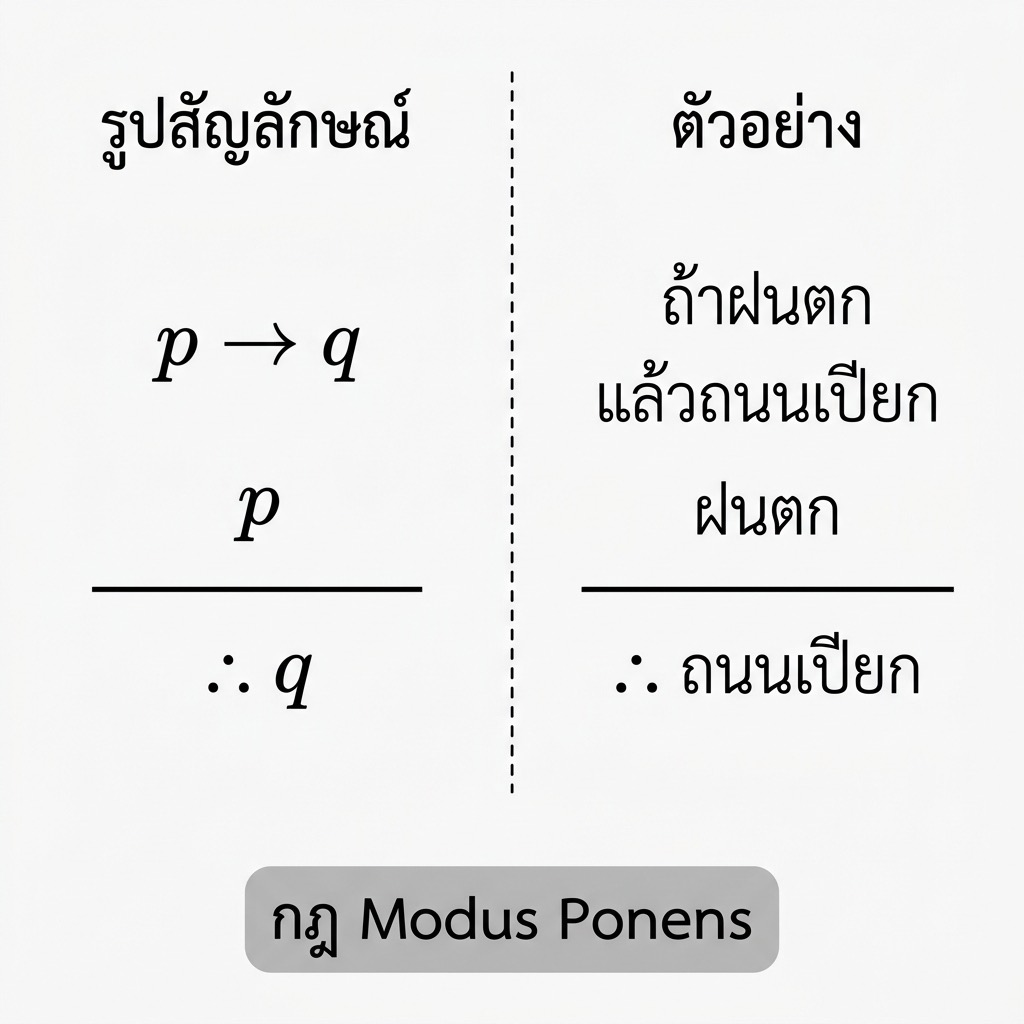
\includegraphics[width=0.85\textwidth]{Figures/07-modus-ponens.png}
    \caption{แผนผังแสดงกฎการอนุมานแบบ Modus Ponens}
    \label{fig:modus-ponens}
\end{figure}

รูปที่ \ref{fig:modus-ponens} แสดงโครงสร้างการอนุมานแบบ Modus Ponens (ละติน: \textit{Modus Ponendo Ponens}) ซึ่งเป็นกฎการอนุมานพื้นฐานในตรรกศาสตร์สัญลักษณ์

\subsubsection{โครงสร้างเชิงตรรกศาสตร์ของ Modus Ponens}
การอนุมานแบบ Modus Ponens ประกอบด้วยข้อตั้งต้น (Premises) 2 ประพจน์ และข้อสรุป (Conclusion) 1 ประพจน์
\begin{enumerate}
    \item ข้อตั้งต้นหลัก (Major Premise) คือประพจน์เงื่อนไข $p \rightarrow q$ ซึ่งระบุความสัมพันธ์ว่าถ้าเงื่อนไขนำ $p$ เกิดขึ้น แล้วเงื่อนไขตาม $q$ จะเกิดตามมา
    \item ข้อตั้งต้นรอง (Minor Premise) คือประพจน์ยืนยันข้อเท็จจริง $p$ ว่าเงื่อนไขนำเกิดขึ้นจริง ($p = T$)
    \item ข้อสรุป (Conclusion) สามารถสรุปผลได้อย่างแน่ชัดว่า $q$ เกิดขึ้นจริง ($\therefore q$)
\end{enumerate}

\subsubsection{การพิสูจน์ความสมเหตุสมผลด้วยตารางค่าความจริง (Tautology Proof)}
การอนุมานแบบ Modus Ponens มีความสมเหตุสมผล (Valid) เนื่องจากรูปแบบประพจน์รวม
\begin{equation}
[(p \rightarrow q) \land p] \rightarrow q
\end{equation}
เป็น \textbf{สัจนิรันดร์ (Tautology)} ซึ่งสามารถพิสูจน์ได้ด้วยตารางค่าความจริงดังตารางที่ \ref{tab:modus-ponens-valid}

\begin{table}[H]
    \centering
    \caption{ตารางค่าความจริงพิสูจน์ความสมเหตุสมผลของ Modus Ponens}
    \label{tab:modus-ponens-valid}
    \begin{tabular}{|c|c|c|c|c|}
        \hline
        $p$ & $q$ & $p \rightarrow q$ & $(p \rightarrow q) \land p$ & $[(p \rightarrow q) \land p] \rightarrow q$ \\ \hline
        \textbf{T} & \textbf{T} & \textbf{T} & \textbf{T} & \textbf{T} \\ \hline
        \textbf{T} & \textbf{F} & \textbf{F} & \textbf{F} & \textbf{T} \\ \hline
        \textbf{F} & \textbf{T} & \textbf{T} & \textbf{F} & \textbf{T} \\ \hline
        \textbf{F} & \textbf{F} & \textbf{T} & \textbf{F} & \textbf{T} \\ \hline
    \end{tabular}
\end{table}

จากตารางที่ \ref{tab:modus-ponens-valid} จะเห็นว่าคอลัมน์สุดท้ายมีค่าความจริงเป็นจริง (T) ในทุกกรณีที่เป็นไปได้ จึงยืนยันได้อย่างเด็ดขาดว่าการให้เหตุผลแบบ Modus Ponens เป็นการอนุมานที่สมเหตุสมผล 100\%

\begin{ex}[การอนุมานแบบ Modus Ponens]
จงหาผลสรุปจากการให้เหตุผลต่อไปนี้ตามหลักเหตุผลทางตรรกศาสตร์
\begin{enumerate}
    \item ถ้าฝนตก แล้วพื้นถนนจะเปียก
    \item ฝนตก
\end{enumerate}
\end{ex}

\begin{solution}
กำหนด $p \equiv \text{ฝนตก}$, $q \equiv \text{พื้นถนนเปียก}$
\[
\begin{array}{r@{\quad}l}
\text{เหตุ 1} & p \rightarrow q\\
\text{เหตุ 2} & p\\
\hline
\therefore & q
\end{array}
\]
นั่นคือ $q \equiv \text{พื้นถนนเปียก}$ \solhere
\end{solution}

จากตัวอย่างจะเห็นว่า เมื่อทราบว่าถ้าฝนตกแล้วพื้นถนนจะเปียก และทราบข้อเท็จจริงว่าฝนตกจริง จึงสรุปได้อย่างแน่ชัดว่าพื้นถนนเปียก

\begin{ex}[การอนุมานแบบ Modus Ponens]
จงหาผลสรุปจากการให้เหตุผลต่อไปนี้ตามหลักเหตุผลทางตรรกศาสตร์
\begin{enumerate}
    \item ถ้าคนรักษาสัญญา แล้วคนนั้นจะได้รับความเชื่อถือ
    \item นาย ก รักษาสัญญา
\end{enumerate}
\end{ex}

\begin{solution}
กำหนด $p \equiv \text{คนรักษาสัญญา}$, $q \equiv \text{ได้รับความเชื่อถือ}$
\[
\begin{array}{r@{\quad}l}
\text{เหตุ 1} & p \rightarrow q\\
\text{เหตุ 2} & p\\
\hline
\therefore & q
\end{array}
\]
นั่นคือ $q \equiv \text{นาย ก ได้รับความเชื่อถือ}$ \solhere
\end{solution}

\subsubsection{การประยุกต์ใช้ในทางวิทยาการคอมพิวเตอร์และปัญญาประดิษฐ์}
กฎ Modus Ponens เป็นหัวใจสำคัญของโครงสร้างคำสั่งและการประมวลผลในวิทยาการคอมพิวเตอร์ เช่น
\begin{itemize}
    \item \textbf{คำสั่งเลือกทำตามเงื่อนไข (Control Flow Statements)} ในการเขียนโปรแกรมด้วยภาษาคอมพิวเตอร์ (เช่น C++, Java, Python) คำสั่งประเภท \texttt{if (condition) \{ action(); \}} อาศัยหลักการของ Modus Ponens โดยตรง กล่าวคือ หากหน่วยประมวลผล (CPU) ตรวจสอบแล้วพบว่าข้อตั้งต้น $p$ (\texttt{condition}) เป็นจริง ($T$) โปรแกรมจะทำการส่งลำดับการทำงานไปประมวลผลคำสั่ง $q$ (\texttt{action()}) ทันที
    \item \textbf{ระบบผู้เชี่ยวชาญและการอนุมานไปข้างหน้า (Forward Chaining in Expert Systems)} ในระบบปัญญาประดิษฐ์แบบอิงกฎ (Rule-Based AI Systems) กลไกการอนุมาน (Inference Engine) จะใช้ Modus Ponens ในการนำข้อเท็จจริงเข้ากระทำกับกฎในฐานความรู้ (Knowledge Base Rules $p \rightarrow q$) เพื่อสร้างข้อสรุปใหม่ๆ ขึ้นมาอย่างเป็นระบบ
\end{itemize}

\subsection{กฎการปฏิเสธ (Modus Tollens)}
\index{Modus Tollens}

Modus Tollens หรือ การปฏิเสธ เป็นรูปแบบการอนุมานที่ใช้ในการปฏิเสธผลลัพธ์เพื่อไปหาการปฏิเสธเงื่อนไขนำ มีรูปแบบดังนี้

\begin{figure}[H]
    \centering
    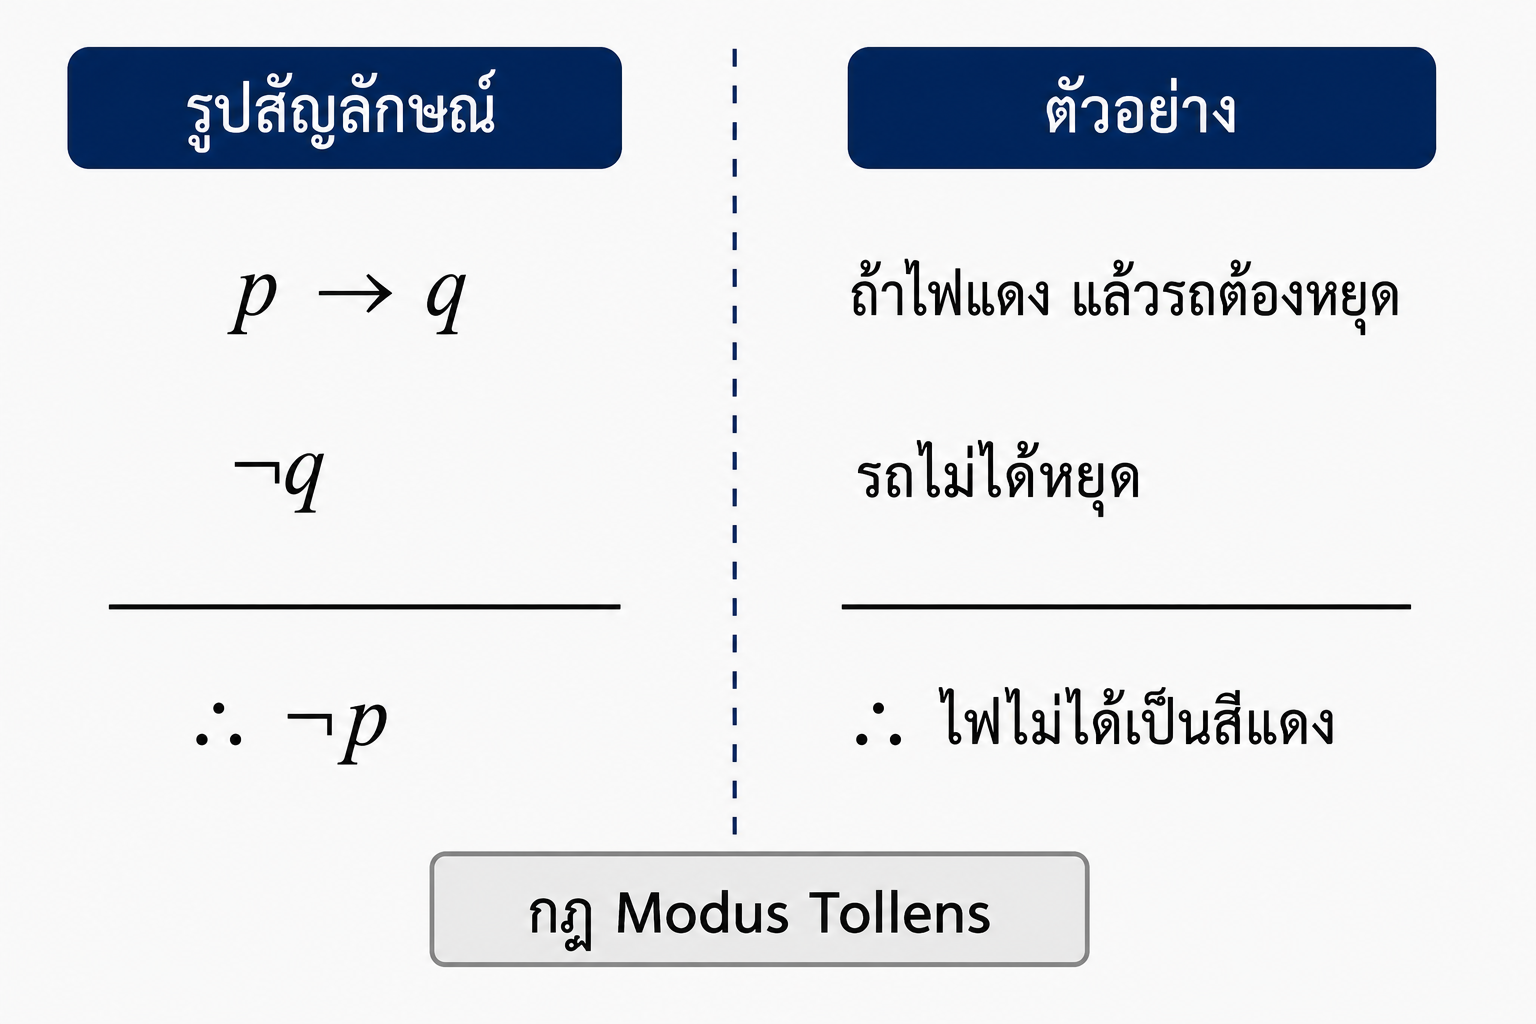
\includegraphics[width=0.85\textwidth]{Figures/08-modus-tollens.png}
    \caption{แผนผังแสดงกฎการอนุมานแบบ Modus Tollens}
    \label{fig:modus-tollens}
\end{figure}

รูปที่ \ref{fig:modus-tollens} แสดงโครงสร้างการอนุมานแบบ Modus Tollens (ละติน: \textit{Modus Tollendo Tollens} แปลว่า ``วิธีแห่งการปฏิเสธเพื่อสรุปผล'') ซึ่งใช้การปฏิเสธเงื่อนไขตามเพื่อสรุปปฏิเสธเงื่อนไขนำ

\subsubsection{โครงสร้างเชิงตรรกศาสตร์ของ Modus Tollens}
การอนุมานแบบ Modus Tollens ประกอบด้วยข้อตั้งต้น 2 ประพจน์ และข้อสรุป 1 ประพจน์
\begin{enumerate}
    \item ข้อตั้งต้นหลัก (Major Premise) คือประพจน์เงื่อนไข $p \rightarrow q$ (ถ้าเกิด $p$ แล้วจะเกิด $q$)
    \item ข้อตั้งต้นรอง (Minor Premise) คือประพจน์ปฏิเสธเงื่อนไขตาม $\neg q$ (ปรากฏว่า $q$ ไม่เกิดขึ้นจริง)
    \item ข้อสรุป (Conclusion) สามารถสรุปผลได้อย่างแน่ชัดว่าเงื่อนไขนำต้องไม่เกิดขึ้นจริง ($\therefore \neg p$)
\end{enumerate}

\subsubsection{การพิสูจน์ความสมเหตุสมผลด้วยตารางค่าความจริง (Tautology Proof)}
การอนุมานแบบ Modus Tollens มีความสมเหตุสมผลเนื่องจากรูปแบบประพจน์รวม
\begin{equation}
[(p \rightarrow q) \land \neg q] \rightarrow \neg p
\end{equation}
เป็น \textbf{สัจนิรันดร์ (Tautology)} ดังแสดงในตารางที่ \ref{tab:modus-tollens-valid}

\begin{table}[H]
    \centering
    \caption{ตารางค่าความจริงพิสูจน์ความสมเหตุสมผลของ Modus Tollens}
    \label{tab:modus-tollens-valid}
    \begin{tabular}{|c|c|c|c|c|c|c|}
        \hline
        $p$ & $q$ & $\neg p$ & $\neg q$ & $p \rightarrow q$ & $(p \rightarrow q) \land \neg q$ & $[(p \rightarrow q) \land \neg q] \rightarrow \neg p$ \\ \hline
        \textbf{T} & \textbf{T} & \textbf{F} & \textbf{F} & \textbf{T} & \textbf{F} & \textbf{T} \\ \hline
        \textbf{T} & \textbf{F} & \textbf{F} & \textbf{T} & \textbf{F} & \textbf{F} & \textbf{T} \\ \hline
        \textbf{F} & \textbf{T} & \textbf{T} & \textbf{F} & \textbf{T} & \textbf{F} & \textbf{T} \\ \hline
        \textbf{F} & \textbf{F} & \textbf{T} & \textbf{T} & \textbf{T} & \textbf{T} & \textbf{T} \\ \hline
    \end{tabular}
\end{table}

จากตารางที่ \ref{tab:modus-tollens-valid} จะเห็นว่าคอลัมน์สุดท้ายมีค่าความจริงเป็นจริง (T) ในทุกกรณี การอนุมานแบบ Modus Tollens จึงสมเหตุสมผล 100\%

\begin{ex}[การอนุมานแบบ Modus Tollens]
จงหาผลสรุปจากการให้เหตุผลต่อไปนี้ตามหลักเหตุผลทางตรรกศาสตร์
\begin{enumerate}
    \item ถ้าฝนตก แล้วพื้นถนนจะเปียก
    \item พื้นถนนไม่เปียก
\end{enumerate}
\end{ex}

\begin{solution}
กำหนด $p \equiv \text{ฝนตก}$, $q \equiv \text{พื้นถนนเปียก}$
\[
\begin{array}{r@{\quad}l}
\text{เหตุ 1} & p \rightarrow q\\
\text{เหตุ 2} & \neg q\\
\hline
\therefore & \neg p
\end{array}
\]
นั่นคือ $\neg p \equiv \text{ฝนไม่ตก}$ \solhere
\end{solution}

จากตัวอย่างจะเห็นว่า เมื่อทราบว่าถ้าฝนตกแล้วพื้นถนนจะเปียก และพื้นถนนไม่เปียก จึงสรุปได้ว่าฝนไม่ตก ทั้งนี้ต้องพิจารณาว่าอาจมีสาเหตุอื่นที่ทำให้พื้นเปียกได้ เช่น รดน้ำต้นไม้

\begin{ex}[การอนุมานแบบ Modus Tollens]
จงหาผลสรุปจากการให้เหตุผลต่อไปนี้ตามหลักเหตุผลทางตรรกศาสตร์
\begin{enumerate}
    \item ถ้าสัตว์เป็นสุนัข แล้วสัตว์นั้นเป็นสัตว์เลี้ยงลูกด้วยนม
    \item สัตว์ตัวนี้ไม่เป็นสัตว์เลี้ยงลูกด้วยนม
\end{enumerate}
\end{ex}

\begin{solution}
กำหนด $p \equiv \text{สัตว์เป็นสุนัข}$, $q \equiv \text{เป็นสัตว์เลี้ยงลูกด้วยนม}$
\[
\begin{array}{r@{\quad}l}
\text{เหตุ 1} & p \rightarrow q\\
\text{เหตุ 2} & \neg q\\
\hline
\therefore & \neg p
\end{array}
\]
นั่นคือ $\neg p \equiv \text{สัตว์ตัวนี้ไม่ใช่สุนัข}$ \solhere
\end{solution}

\subsubsection{การประยุกต์ใช้ในทางวิทยาการคอมพิวเตอร์และซอฟต์แวร์}
กฎ Modus Tollens มีบทบาทสำคัญในการทดสอบซอฟต์แวร์และการค้นหาข้อผิดพลาด (Debugging \& Fault Isolation) เช่น
\begin{itemize}
    \item \textbf{การทดสอบหน่วย (Unit Testing Verification)} หากกำหนดข้อตั้งต้นว่า ``ถ้าอัลกอริทึมทำงานถูกต้อง ($p$) แล้วจะได้ผลลัพธ์ $q$'' แต่เมื่อทดสอบ (Unit Test) พบว่าผลลัพธ์ที่ได้ไม่ใช่ $q$ ($\neg q$) นักพัฒนาสามารถสรุปด้วยกฎ Modus Tollens ได้ทันทีว่าอัลกอริทึมมีความผิดพลาดหรือมีบักเกิดขึ้น ($\neg p$)
    \item \textbf{การอนุมานย้อนกลับในระบบปัญญาประดิษฐ์ (Backward Chaining)} ในระบบสืบค้นและวินิจฉัยปัญหา (Diagnostic Expert Systems) กลไกจะใช้ Modus Tollens ในการตัดสาเหตุที่ไม่เกี่ยวข้องออก เมื่อผลลัพธ์อันไม่พึงประสงค์ไม่ได้เกิดขึ้น
\end{itemize}

\subsection{การอ้างเหตุผลแบบมีเงื่อนไข (Hypothetical Syllogism)}
\index{Hypothetical Syllogism}

Hypothetical Syllogism หรือ การอ้างเหตุผลแบบมีเงื่อนไข เป็นรูปแบบการอนุมานที่เชื่อมโยงเงื่อนไขหลายข้อเข้าด้วยกัน มีรูปแบบดังนี้

\begin{enumerate}
    \item ถ้า $p$ แล้ว $q$ โดยมีข้อตั้งต้นที่ 1
    \item ถ้า $q$ แล้ว $r$ และข้อตั้งต้นที่ 2
    \item $\therefore$ ถ้า $p$ แล้ว $r$ ผลสรุปคือ
\end{enumerate}

อ่านได้ว่า ถ้า $p$ นำไปสู่ $q$ และ $q$ นำไปสู่ $r$ แล้ว $p$ จะนำไปสู่ $r$ โดยตรง หลักการนี้เรียกว่า การถ่ายโอนเงื่อนไข (Conditional Transitivity) ซึ่งมีความสำคัญในการสร้างการให้เหตุผลที่ซับซ้อน

\begin{ex}[การอนุมานแบบ Hypothetical Syllogism]
จงหาผลสรุปจากการให้เหตุผลต่อไปนี้ตามหลักเหตุผลทางตรรกศาสตร์
\begin{enumerate}
    \item ถ้าฝนตก แล้วถนนจะเปียก
    \item ถ้าถนนเปียก แล้วรถจะลื่น
\end{enumerate}
\end{ex}

\begin{solution}
กำหนด $p \equiv \text{ฝนตก}$, $q \equiv \text{ถนนเปียก}$, $r \equiv \text{รถจะลื่น}$
\[
\begin{array}{r@{\quad}l}
\text{เหตุ 1} & p \rightarrow q\\
\text{เหตุ 2} & q \rightarrow r\\
\hline
\therefore & p \rightarrow r
\end{array}
\]
นั่นคือ $p \rightarrow r \equiv \text{ถ้าฝนตก แล้วรถจะลื่น}$ \solhere
\end{solution}

ตัวอย่างนี้แสดงให้เห็นว่าสามารถเชื่อมโยงเงื่อนไขหลายข้อเข้าด้วยกันเพื่อสร้างเงื่อนไขใหม่ที่ซับซ้อนขึ้น

ในการเขียนโปรแกรม Hypothetical Syllogism สามารถใช้ในการตรวจสอบเงื่อนไขแบบต่อเนื่อง เช่น ถ้า input ถูกต้อง แล้ว process จะทำงาน ถ้า process ทำงาน แล้ว output จะถูกสร้าง ดังนั้นถ้า input ถูกต้อง แล้ว output จะถูกสร้าง

\subsection{การอ้างเหตุผลแบบแยก (Disjunctive Syllogism)}
\index{Disjunctive Syllogism}

Disjunctive Syllogism หรือ การอ้างเหตุผลแบบแยก เป็นรูปแบบการอนุมานที่ใช้กับประพจน์ที่เชื่อมด้วย OR มีรูปแบบดังนี้

\begin{enumerate}
    \item $p \lor q$ โดยมีข้อตั้งต้นที่ 1
    \item $\neg p$ และข้อตั้งต้นที่ 2
    \item $\therefore q$ ผลสรุปคือ
\end{enumerate}

อ่านได้ว่า ถ้า $p$ หรือ $q$ เป็นจริง และ $p$ เป็นเท็จ แล้ว $q$ ต้องเป็นจริง หลักการคือเมื่อทราบว่าอย่างน้อยหนึ่งในสองอย่างเป็นจริง และทราบว่าอย่างหนึ่งเป็นเท็จ อีกอย่างหนึ่งต้องเป็นจริง

\begin{ex}[การอนุมานแบบ Disjunctive Syllogism]
จงหาผลสรุปจากการให้เหตุผลต่อไปนี้ตามหลักเหตุผลทางตรรกศาสตร์
\begin{enumerate}
    \item นาย ก อยู่บ้านหรืออยู่ที่ทำงาน
    \item นาย ก ไม่ได้อยู่ที่ทำงาน
\end{enumerate}
\end{ex}

\begin{solution}
กำหนด $p \equiv \text{นาย ก อยู่บ้าน}$, $q \equiv \text{นาย ก อยู่ที่ทำงาน}$
\[
\begin{array}{r@{\quad}l}
\text{เหตุ 1} & p \lor q\\
\text{เหตุ 2} & \neg q\\
\hline
\therefore & p
\end{array}
\]
นั่นคือ $p \equiv \text{นาย ก อยู่บ้าน}$ \solhere
\end{solution}

ในการเขียนโปรแกรม Disjunctive Syllogism สามารถใช้ในการตรวจสอบสถานะและการตัดสินใจ เช่น ถ้า error flag เป็น E1 หรือ E2 และตรวจพบว่า error flag ไม่ใช่ E1 แล้ว error flag ต้องเป็น E2

\section{การพิสูจน์ด้วยตารางค่าความจริง}
\index{การพิสูจน์!ตารางค่าความจริง}
\zlabel{sec:truth-table-proof}

\begin{ex}[การสร้างระบบการตัดสินใจ]
\label{ex:decision-tree-logic}
จงใช้ตรรกะประพจน์ในการสร้างระบบการตัดสินใจแบบง่าย (Decision Tree) สำหรับการอนุมัติสินเชื่อ โดยมีเงื่อนไขดังต่อไปนี้
\begin{enumerate}
    \item ถ้าผู้สมัครมีรายได้สูงกว่า 50,000 บาทต่อเดือน และไม่มีหนี้ค้างชำระ จะได้รับอนุมัติ
    \item ถ้าผู้สมัครมีรายได้สูงกว่า 50,000 บาทต่อเดือน แต่มีหนี้ค้างชำระ จะต้องพิจารณาเพิ่มเติม
    \item ถ้าผู้สมัครมีรายได้ต่ำกว่าหรือเท่ากับ 50,000 บาทต่อเดือน จะไม่ได้รับอนุมัติ
\end{enumerate}
จงเขียนประพจน์เชิงประกอบและตารางค่าความจริงสำหรับการตัดสินใจนี้
\end{ex}

\begin{solution}
กำหนดประพจน์
\begin{align*}
I &\equiv \text{ผู้สมัครมีรายได้สูงกว่า 50,000 บาทต่อเดือน}\\
D &\equiv \text{ผู้สมัครมีหนี้ค้างชำระ}\\
A &\equiv \text{ได้รับอนุมัติสินเชื่อ}\\
P &\equiv \text{ต้องพิจารณาเพิ่มเติม}\\
N &\equiv \text{ไม่ได้รับอนุมัติสินเชื่อ}
\end{align*}
จากเงื่อนไขทั้งสามเขียนประพจน์เชิงประกอบได้เป็น
\begin{align*}
A &\equiv I \land \neg D \quad (\text{เงื่อนไข 1})\\
P &\equiv I \land D \quad (\text{เงื่อนไข 2})\\
N &\equiv \neg I \quad (\text{เงื่อนไข 3})
\end{align*}

\begin{center}
\begin{tabular}{|c|c|c|c|c|c|}
\hline
$I$ & $D$ & $A$ & $P$ & $N$ & ผลการตัดสินใจ \\
\hline
\text{T} & \text{T} & \text{F} & \text{T} & \text{F} & พิจารณาเพิ่มเติม \\
\text{T} & \text{F} & \text{T} & \text{F} & \text{F} & อนุมัติ \\
\text{F} & \text{T} & \text{F} & \text{F} & \text{T} & ไม่อนุมัติ \\
\text{F} & \text{F} & \text{F} & \text{F} & \text{T} & ไม่อนุมัติ \\
\hline
\end{tabular}
\end{center}

จากตารางค่าความจริง ระบบจะอนุมัติเมื่อ $I \land \neg D$ เป็นจริง, พิจารณาเพิ่มเติมเมื่อ $I \land D$ และไม่อนุมัติเมื่อ $\neg I$ \solhere
\end{solution}

ในการวิเคราะห์ประพจน์เชิงประกอบที่ซับซ้อน การใช้ตารางค่าความจริงเป็นวิธีการที่เป็นระบบและแม่นยำในการตรวจสอบความสมมูลหรือความถูกต้องของประพจน์ การพิสูจน์ด้วยตารางค่าความจริงอาจใช้เวลานานหากประพจน์มีตัวแปรหลายตัว แต่ให้ผลลัพธ์ที่แน่นอนและตรวจสอบได้

การใช้ตารางค่าความจริงในการพิสูจน์มีหลายวัตถุประสงค์ ได้แก่ การตรวจสอบว่าประพจน์เป็นสัจนิรันดร์หรือไม่ การตรวจสอบว่าประพจน์สองประพจน์สมมูลกันหรือไม่ และการตรวจสอบความสมเหตุสมผลของการให้เหตุผล ในการพิสูจน์ว่าประพจน์สองประพจน์ $P$ และ $Q$ สมมูลกัน ($P \equiv Q$) จะต้องสร้างตารางค่าความจริงสำหรับทั้งสองประพจน์ แล้วเปรียบเทียบคอลัมน์ของผลลัพธ์ ถ้าค่าความจริงเหมือนกันทุกกรณี แสดงว่าประพจน์ทั้งสองสมมูลกัน

ในการพิสูจน์ว่าการให้เหตุผลสมเหตุสมผล โดยการเขียนข้อตั้งต้นทั้งหมดเชื่อมด้วย AND แล้วเชื่อมกับเงื่อนไขนำของผลสรุปด้วย $\rightarrow$ ถ้าประพจน์ที่ได้เป็นสัจนิรันดร์ แสดงว่าการให้เหตุผลนั้นสมเหตุสมผล

\begin{thrm}[ความสมมูลระหว่าง Implication กับ Disjunction]
\index{สมมูล!implication-disjunction}
สำหรับทุกประพจน์ $p$ และ $q$ จะได้ว่า
\begin{equation}
p \rightarrow q \equiv \neg p \lor q
\end{equation}
โดยที่ $p$ และ $q$ เป็นประพจน์ใดๆ, $\neg p$ คือนิเสธของ $p$ ที่กลับค่าความจริงจากจริงเป็นเท็จหรือจากเท็จเป็นจริง และ $\lor$ คือตัวเชื่อมแบบหรือที่จะเป็นจริงเมื่ออย่างน้อยหนึ่งประพจน์เป็นจริง นั่นคือประพจน์เชิงเงื่อนไขสมมูลกับการเชื่อมแบบหรือระหว่างนิเสธของเงื่อนไขนำกับเงื่อนไขตาม
\end{thrm}

\begin{proof}
\index{พิสูจน์!implication-disjunction}
พิจารณาตารางค่าความจริงสำหรับ $p \rightarrow q$ และ $\neg p \lor q$ ดังแสดงในตารางที่ \ref{tab:implies-equiv-proof}

สำหรับแถวที่ 1 เมื่อ $p = T$ และ $q = T$ จะได้ $p \rightarrow q = T$ และ $\neg p \lor q = F \lor T = T$ ค่าเท่ากัน

สำหรับแถวที่ 2 เมื่อ $p = T$ และ $q = F$ จะได้ $p \rightarrow q = F$ และ $\neg p \lor q = F \lor F = F$ ค่าเท่ากัน

สำหรับแถวที่ 3 เมื่อ $p = F$ และ $q = T$ จะได้ $p \rightarrow q = T$ และ $\neg p \lor q = T \lor T = T$ ค่าเท่ากัน

สำหรับแถวที่ 4 เมื่อ $p = F$ และ $q = F$ จะได้ $p \rightarrow q = T$ และ $\neg p \lor q = T \lor F = T$ ค่าเท่ากัน

เนื่องจากทั้ง 4 กรณีให้ค่าเท่ากันทุกแถว จึงสรุปได้ว่า $p \rightarrow q \equiv \neg p \lor q$ ตามที่ต้องการพิสูจน์
\end{proof}

ตัวอย่างการพิสูจน์ พิสูจน์ว่า $p \rightarrow q$ และ $\neg p \lor q$ มีค่าความจริงเหมือนกัน (สมมูลกัน)

\begin{table}[h]
    \centering
\caption{ตารางพิสูจน์ว่า $p \rightarrow q \equiv \neg p \lor q$}
\label{tab:implies-equiv-proof}
    \begin{tabular}{|c|c|c|c|c|c|}
        \hline
        \textbf{$p$} & \textbf{$q$} & \textbf{$p \rightarrow q$} & \textbf{$\neg p$} & \textbf{$\neg p \lor q$} & \textbf{การสมมูลกัน} \\ \hline
        T & T & T & F & T & \checkmark \\ \hline
        T & F & F & F & F & \checkmark \\ \hline
        F & T & T & T & T & \checkmark \\ \hline
        F & F & T & T & T & \checkmark \\ \hline
    \end{tabular}
\end{table}

ตารางที่ \ref{tab:implies-equiv-proof} แสดงให้เห็นว่าคอลัมน์ $p \rightarrow q$ และ $\neg p \lor q$ มีค่าเหมือนกันทุกแถว จึงสรุปได้ว่า $p \rightarrow q \equiv \neg p \lor q$

ผลลัพธ์นี้มีความสำคัญอย่างยิ่งในการแปลงประพจน์เชิงเงื่อนไขให้อยู่ในรูปแบบที่ใช้เฉพาะ AND, OR, NOT ซึ่งมีประโยชน์ในการออกแบบวงจรดิจิทัลและการเขียนโปรแกรม

\section{สรุป}
\index{สรุป}
\zlabel{sec:summary}

บทนี้ได้กล่าวถึงพื้นฐานของตรรกศาสตร์ (Logic) ซึ่งเป็นรากฐานสำคัญของวิทยาการคอมพิวเตอร์และคณิตศาสตร์เชิงคำนวณ เนื้อหาครอบคลุมหัวข้อสำคัญหลายประการ โดยเริ่มจากความหมายและความสำคัญของตรรกศาสตร์ที่มีบทบาทในการให้เหตุผลอย่างมีระบบ ต่อด้วยประพจน์ (Propositions) ซึ่งเป็นหน่วยพื้นฐานที่สุดของตรรกศาสตร์ที่สามารถระบุค่าความจริงได้ และตัวเชื่อมประพจน์ (Logical Connectives) ทั้ง 5 ตัว ได้แก่ นิเสธ ($\neg$) การเชื่อมแบบและ ($\land$) การเชื่อมแบบหรือ ($\lor$) การเชื่อมแบบถ้า...แล้ว ($\rightarrow$) และการเชื่อมแบบก็ต่อเมื่อ ($\leftrightarrow$) ตารางค่าความจริง (Truth Tables) เป็นเครื่องมือสำคัญในการวิเคราะห์ค่าความจริงของประพจน์เชิงประกอบ ช่วยให้สามารถตรวจสอบค่าความจริงของประพจน์ที่ซับซ้อนได้อย่างเป็นระบบ นอกจากนี้ยังได้ศึกษาประเภทของประพจน์เชิงประกอบ ได้แก่ สัจนิรันดร์ (Tautology) ซึ่งเป็นจริงทุกกรณี ข้อขัดแย้ง (Contradiction) ซึ่งเป็นเท็จทุกกรณี และประพจน์กลาง (Contingency) ซึ่งมีค่าความจริงขึ้นกับกรณี การอนุมาน (Inference Rules) เป็นกฎที่ใช้ในการสรุปผลอย่างมีตรรกะ ประกอบด้วย Modus Ponens, Modus Tollens, Hypothetical Syllogism และ Disjunctive Syllogism ซึ่งมีความสำคัญในการให้เหตุผลแบบนิรนัยและการเขียนโปรแกรม ทั้งหมดนี้เป็นพื้นฐานที่จำเป็นสำหรับการศึกษาบทต่อไปและการนำไปประยุกต์ใช้ในงานด้านวิทยาการคอมพิวเตอร์~\cite{rosen2019discrete}

\clearpage
\section{แบบฝึกหัดท้ายบท}

\begin{exercise}
จงพิจารณาว่าข้อความต่อไปนี้เป็นประพจน์หรือไม่ ถ้าเป็นให้ระบุค่าความจริง
\begin{enumerate}
    \item $3 + 5 = 8$
    \item $x > 10$
    \item กรุณาปิดประตู
    \item $7$ เป็นจำนวนคู่
    \item พรุ่งนี้จะเป็นวันพระ
    \item ความรักคือสิ่งสวยงาม
    \item $2^2 = 4$
\end{enumerate}
\end{exercise}

\begin{exercise}
จงสร้างตารางค่าความจริงของประพจน์ต่อไปนี้
\begin{enumerate}
    \item $p \land \neg q$
    \item $\neg p \lor q$
    \item $(p \rightarrow q) \land (q \rightarrow p)$
    \item $(p \lor q) \rightarrow r$
    \item $\neg(p \land q) \leftrightarrow (\neg p \lor \neg q)$
\end{enumerate}
\end{exercise}

\begin{exercise}
จงพิสูจน์ว่าประพจน์ต่อไปนี้เป็นสัจนิรันดร์หรือไม่ โดยใช้ตารางค่าความจริง
\begin{enumerate}
    \item $(p \rightarrow q) \lor (q \rightarrow p)$
    \item $(p \land q) \rightarrow p$
    \item $p \lor \neg p$
    \item $(p \rightarrow q) \leftrightarrow (\neg p \lor q)$
\end{enumerate}
\end{exercise}

\begin{exercise}
จงพิสูจน์ว่าประพจน์ต่อไปนี้เป็นข้อขัดแย้งหรือไม่
\begin{enumerate}
    \item $p \land \neg p$
    \item $\neg(p \lor \neg p)$
    \item $(p \rightarrow q) \land (p \land \neg q)$
\end{enumerate}
\end{exercise}

\begin{exercise}
จงใช้การอนุมานแบบ Modus Ponens หรือ Modus Tollens เพื่อหาผลสรุป
\begin{enumerate}
    \item ถ้าวันนี้ฝนตก แล้วฉันจะไม่ออกไปข้างนอก วันนี้ฝนตก $\therefore$ ?
    \item ถ้าข้าพเจ้าสอบผ่าน แล้วข้าพเจ้าจะดีใจ ข้าพเจ้าไม่ดีใจ $\therefore$ ?
    \item ถ้าผู้สมัครมีประสบการณ์ แล้วผู้สมัครจะได้รับการคัดเลือก ผู้สมัครไม่ได้รับการคัดเลือก $\therefore$ ?
\end{enumerate}
\end{exercise}

\begin{exercise}
จงตรวจสอบว่าประพจน์สมมูลกันหรือไม่
\begin{enumerate}
    \item $p \rightarrow q$ และ $\neg p \lor q$
    \item $\neg(p \land q)$ และ $\neg p \lor \neg q$ (กฎของ De Morgan ข้อที่ 1)
    \item $\neg(p \lor q)$ และ $\neg p \land \neg q$ (กฎของ De Morgan ข้อที่ 2)
    \item $p \leftrightarrow q$ และ $(p \rightarrow q) \land (q \rightarrow p)$
\end{enumerate}
\end{exercise}

\begin{exercise}
จงเขียนประพจน์ในรูปแบบเชิงสัญลักษณ์ โดยกำหนดให้ $p$ แทนฝนตก, $q$ แทนพื้นเปียก, และ $r$ แทนฉันจะอยู่บ้าน
\begin{enumerate}
    \item ถ้าฝนตก แล้วฉันจะอยู่บ้าน
    \item ฝนตกและพื้นเปียก
    \item ถ้าฝนไม่ตก แล้วฉันจะไม่อยู่บ้าน
    \item ฉันจะอยู่บ้านก็ต่อเมื่อฝนตกหรือพื้นเปียก
\end{enumerate}
\end{exercise}

\begin{exercise}
ให้นักศึกษาอธิบายความแตกต่างระหว่างสัจนิรันดร์ ข้อขัดแย้ง และประพจน์กลาง พร้อมยกตัวอย่างประกอบแต่ละประเภทอย่างน้อย 2 ตัวอย่าง
\end{exercise}

\clearpage
\section{เฉลยแบบฝึกหัด}
ในส่วนนี้แสดงเฉลยอย่างย่อสำหรับแบบฝึกหัดท้ายบทตามลำดับข้างต้น เพื่อให้ผู้เรียนใช้ตรวจคำตอบของตนเอง

\begin{enumerate}
    \item ระบุประพจน์และค่าความจริง (ก) เป็นประพจน์ ค่าจริง; (ข) ไม่เป็นประพจน์ เพราะมีตัวแปร $x$; (ค) ไม่เป็นประพจน์ เป็นประโยคคำสั่ง; (ง) เป็นประพจน์ ค่าเท็จ ($7$ เป็นจำนวนคี่); (จ) เป็นประโยคบอกเล่าเกี่ยวกับอนาคต ซึ่งในตรรกศาสตร์คลาสสิกมักถือว่าเป็นประพจน์ได้หากเหตุการณ์นั้นมีค่าความจริงแน่นอน แม้ผู้พูดจะยังไม่ทราบค่าความจริงในขณะกล่าว; (ฉ) ไม่เป็นประพจน์ เป็นข้อคิดเห็นเชิงค่านิยม; (ช) เป็นประพจน์ ค่าจริง
    \item ตารางค่าความจริง ใช้ $p,q,r \in \{T,F\}$ สร้างตารางขนาด $2^n$ แถว เช่น $p\land\neg q$ มีค่าจริงเฉพาะแถว $p=T, q=F$; $(p\rightarrow q)\land(q\rightarrow p)$ มีค่าจริงเมื่อ $p$ และ $q$ มีค่าตรงกัน (สมมูล $p\leftrightarrow q$)
    \item สัจนิรันดร์ (ก) เป็นสัจนิรันดร์ เพราะตรวจทุกแถวให้ค่าจริง; (ข) เป็นสัจนิรันดร์ (Law of Simplification); (ค) เป็นสัจนิรันดร์ (Law of Excluded Middle); (ง) เป็นสัจนิรันดร์ เพราะ $p\rightarrow q \equiv \neg p \lor q$
    \item ข้อขัดแย้ง (ก) เป็นข้อขัดแย้ง เพราะ $p\land\neg p$ เป็นเท็จเสมอ; (ข) เป็นข้อขัดแย้ง เพราะ $p\lor\neg p$ เป็นจริงเสมอ จึงนิเสธเป็นเท็จเสมอ; (ค) เป็นข้อขัดแย้ง เพราะถ้า $p\rightarrow q$ จริงและ $p$ จริง $q$ ต้องจริง ขัดกับ $\neg q$
    \item \textbf{Modus Ponens/Tollens:} (ก) สรุปว่า "ฉันจะไม่ออกไปข้างนอก" (Modus Ponens); (ข) สรุปว่า "ข้าพเจ้าสอบไม่ผ่าน" (Modus Tollens); (ค) สรุปว่า "ผู้สมัครไม่มีประสบการณ์" (Modus Tollens)
    \item ความสมมูล (ก) สมมูล โดยตารางค่าความจริง; (ข) และ (ค) สมมูล (กฎ De Morgan); (ง) สมมูล จากนิยามของไบคอนดิชันแนล
    \item ประพจน์เชิงสัญลักษณ์ (ก) $p\rightarrow r$; (ข) $p\land q$; (ค) $\neg p \rightarrow \neg r$; (ง) $r \leftrightarrow (p\lor q)$
    \item ความแตกต่าง สัจนิรันดร์คือประพจน์ที่จริงทุกการประเมิน (เช่น $p\lor\neg p$); ข้อขัดแย้งคือประพจน์ที่เท็จทุกการประเมิน (เช่น $p\land\neg p$); ประพจน์กลางคือมีทั้งจริงและเท็จ (เช่น $p\land q$, $p\rightarrow q$)
\end{enumerate}

\QAChapter
\begin{enumerate}
    \item จงระบุว่าข้อความต่อไปนี้เป็นประพจน์หรือไม่ พร้อมระบุค่าความจริงของข้อที่เป็นประพจน์ ดังนี้ (ก) กรุงเทพฯ เป็นเมืองหลวงของไทย (ข) $x + 3 = 10$ (ค) กรุณาปิดไฟ (ง) $3 \times 3 = 10$
    \item กำหนดให้ $p$ แทนฝนตก และ $q$ แทนถนนเปียก จงสร้างตารางค่าความจริงของ $p \rightarrow q$ และ $\neg p \lor q$ แล้วสรุปว่าทั้งสองประพจน์สมมูลกันหรือไม่
    \item จงพิสูจน์ด้วยตารางค่าความจริงว่า $(p \land q) \lor (p \land \neg q) \equiv p$
    \item จงจำแนกประพจน์ต่อไปนี้ว่าเป็นสัจนิรันดร์ ข้อขัดแย้ง หรือประพจน์กลาง (ก) $p \lor \neg p$ (ข) $p \land \neg p$ (ค) $(p \rightarrow q) \rightarrow (\neg q \rightarrow \neg p)$
    \item จงหา converse, inverse และ contrapositive ของประพจน์ "ถ้า $n$ หารด้วย 4 ลงตัว แล้ว $n$ หารด้วย 2 ลงตัว"
    \item จงใช้กฎ Modus Ponens สรุปผลจาก: ถ้าโปรแกรมไม่มีบัก แล้วโปรแกรมทำงานถูกต้อง, โปรแกรมไม่มีบัก
    \item จงตรวจสอบว่าการให้เหตุผลต่อไปนี้สมเหตุสมผลหรือไม่โดยใช้ตารางค่าความจริง จากสมมติฐาน $p \rightarrow q$ และ $\neg q$ สรุปได้ว่า $\neg p$
    \item จงประยุกต์ใช้ตรรกศาสตร์เขียนเงื่อนไขการรับสมัครงานต่อไปนี้เป็นสูตรตรรกศาสตร์ "ผู้สมัครต้องมีวุฒิปริญญาตรีและประสบการณ์ไม่น้อยกว่า 2 ปี หรือมีวุฒิปริญญาโท"
\end{enumerate}

\newpage
\sheetChapter{ตรรกศาสตร์ (Logic)}
\section*{วัตถุประสงค์}
\begin{enumerate}
    \item เพื่อให้ผู้เรียนอธิบายความหมายของประพจน์และค่าความจริงได้
    \item เพื่อให้ผู้เรียนสร้างและวิเคราะห์ตารางค่าความจริงสำหรับประพจน์เชิงประกอบได้
    \item เพื่อให้ผู้เรียนตรวจสอบความสมมูลทางตรรกศาสตร์และจำแนกประเภทของประพจน์ได้
    \item เพื่อให้ผู้เรียนประยุกต์ใช้กฎการอนุมานในการให้เหตุผลแบบนิรนัยได้
\end{enumerate}
\section*{คำชี้แจง} ให้ผู้เรียนศึกษาเนื้อหาบทตรรกศาสตร์ แล้วตอบคำถามต่อไปนี้
\begin{enumerate}
    \item จงอธิบายความแตกต่างระหว่างประพจน์เชิงเดี่ยวและประพจน์เชิงประกอบ พร้อมยกตัวอย่างอย่างละ 2 ข้อ
    \Pointilles{3}
    \item จงสร้างตารางค่าความจริงของ $p \rightarrow (q \lor \neg r)$ โดยใช้ตัวแปร $p$, $q$, $r$
    \Pointilles{3}
    \item จงพิสูจน์ว่า $p \leftrightarrow q \equiv (p \rightarrow q) \land (q \rightarrow p)$ ด้วยตารางค่าความจริง
    \Pointilles{3}
    \item จงอธิบายความหมายของ Modus Ponens และ Modus Tollens พร้อมยกตัวอย่างสถานการณ์จริงอย่างละ 1 ตัวอย่าง
    \Pointilles{3}
    \item จงตรวจสอบว่า $[(p \rightarrow q) \land (q \rightarrow r)] \rightarrow (p \rightarrow r)$ เป็นสัจนิรันดร์หรือไม่
    \Pointilles{3}
    \item จงอธิบายการเชื่อมโยงระหว่างตรรกศาสตร์กับการเขียนโปรแกรม พร้อมยกตัวอย่างการใช้ตัวเชื่อมตรรกะในคำสั่ง \texttt{if-else}
    \Pointilles{3}
\end{enumerate}
